\documentclass{article}



%\PassOptionsToPackage{numbers, compress}{natbib}
% before loading neurips_2026
\PassOptionsToPackage{numbers,compress}{natbib}
\usepackage{neurips_2026}

\usepackage[utf8]{inputenc}
\usepackage[T1]{fontenc}
\usepackage{url}
\usepackage{booktabs}
\usepackage{amsfonts}
\usepackage{amsmath}
\usepackage{amssymb}
\usepackage{mathtools}
\usepackage{multirow}
\usepackage{graphicx}
\usepackage{nicefrac}
\usepackage{microtype}
\usepackage[table]{xcolor}
\usepackage{array}
\usepackage{wrapfig}
\usepackage{placeins}
\usepackage{capt-of}
\usepackage{rotating}
\usepackage{hyperref}
\usepackage{pdflscape}
\usepackage{adjustbox}

\usepackage{algorithm}
\usepackage{algpseudocode}

\newcommand{\rot}[1]{\rotatebox[origin=c]{65}{#1}}

\newcommand{\method}{\textsc{ATLAS}}
\newcommand{\fullmethod}{\textbf{A}daptive \textbf{T}est-time \textbf{L}earning \textbf{A}cross \textbf{S}cenarios}
\newcommand{\core}{\textsc{CORE}}
\newcommand{\fullcore}{corroborative entity selection}
\newcommand{\care}{\textsc{CARE}}
\newcommand{\fullcare}{drift-anchored conservative adaptation}
\newcommand{\sane}{\textsc{SANE}}
\newcommand{\fullsane}{entity-scale normalization}
\newcommand{\atlasloss}{\textsc{ATLAS} loss}
\newcommand{\avg}{Avg.}
\newcommand{\pending}{\textemdash}


\setlength{\parindent}{0pt}

\newcommand{\std}[1]{$_{\pm #1}$}
\newcommand{\res}[2]{#1\std{#2}}
\newcommand{\best}[2]{\textbf{#1}\std{#2}}
\newcommand{\ulres}[2]{\underline{#1}\std{#2}}
\newcommand{\gain}[1]{\textcolor{green!50!black}{#1}}


\title{\method: Adaptive Test-time Learning Across Scenarios}
% \title{\textsc{ATLAS}: Adaptive Test-Time Learning with Anchored Support Across Scenarios}

\begin{document}

\maketitle

\begin{abstract}
Test-time adaptation (TTA) updates deployed models from unlabeled target inputs, but evidence that is useful in one deployment setting can become unreliable under a different stream, model interface, or adaptation entity. We present \textbf{A}daptive \textbf{T}est-time \textbf{L}earning \textbf{A}cross \textbf{S}cenarios (\textbf{ATLAS}), a reliability-oriented TTA formulation organized around three design principles. \textbf{CORE} selects image, pixel, or prompt-view entities only when source, raw, and semantics-preserving views provide corroborating evidence while a destroy view tests structural sensitivity. \textbf{CARE} anchors accepted updates using either source-relative clipping or class-centered support. \textbf{SANE} normalizes the loss by selected entities rather than the raw tensor size. We instantiate these principles with task-specific parameter scopes, gates, and optimization protocols for corruption robustness, natural shifts, non-i.i.d. streams, dense prediction, and episodic prompt adaptation. Under this five-level evaluation, ATLAS reaches $68.8\%$ on CIFAR-100-C continual adaptation, $65.14\%$ on ViT-B/16 ImageNet-C continual adaptation, and $64.2\%$ OOD average accuracy for CLIP ViT-B/16 prompt adaptation with CoOp initialization. Component ablations attribute the classification gains to evidence selection and anchoring, while the segmentation ablation shows that selected-entity normalization is necessary in the evaluated dense-prediction setting. These results support the three reliability principles across the studied interfaces without assuming one numerical recipe for every scenario. Part of the core code is included in the supplementary materials.
\end{abstract}

\section{Introduction}
Existing test-time adaptation methods often fail when deployment shifts across streams, backbones, or tasks. In TTA, a source-trained model updates itself from unlabeled target inputs at inference. This source-free setting is used for corruptions, covariate shift, natural shifts, dense prediction, and prompt-only VLM adaptation~\citep{schneider2020covariateshift,wang2021tent,niu2022eata,wang2022cotta,niu2023sar,yuan2023rotta,lee2024deyo,karmanov2024tda,farina2024zero,niu2024foa,dai2025freetta,sheng2025ttavlm,ma2025adadem,duan2025lifelong,ma2025surgeon,tan2025eatac}. Its central problem is reliability: weak target evidence can corrupt the next model state.

Recent methods use confidence filters, regularization, teachers, memories, gradient constraints, or prompt tuning, and usually instantiate these safeguards for a particular model or task interface. Our experiments expose corresponding changes in failure behavior: a filter that works for reset corruption evaluation can fail under a non-i.i.d. stream, and image-level loss scaling does not directly specify how dense pixels or prompt views should contribute. We therefore study a reliability decomposition with three linked operations: \core{} selects corroborated evidence, \care{} anchors accepted updates against drift, and \sane{} normalizes the update by selected entities. ATLAS instantiates this decomposition separately for each evaluated interface; it does not assume that the trainable parameters, gates, optimizer, or numerical settings are identical across tasks.

\begin{wrapfigure}{r}{0.48\textwidth}
\vspace{-10pt}
\centering
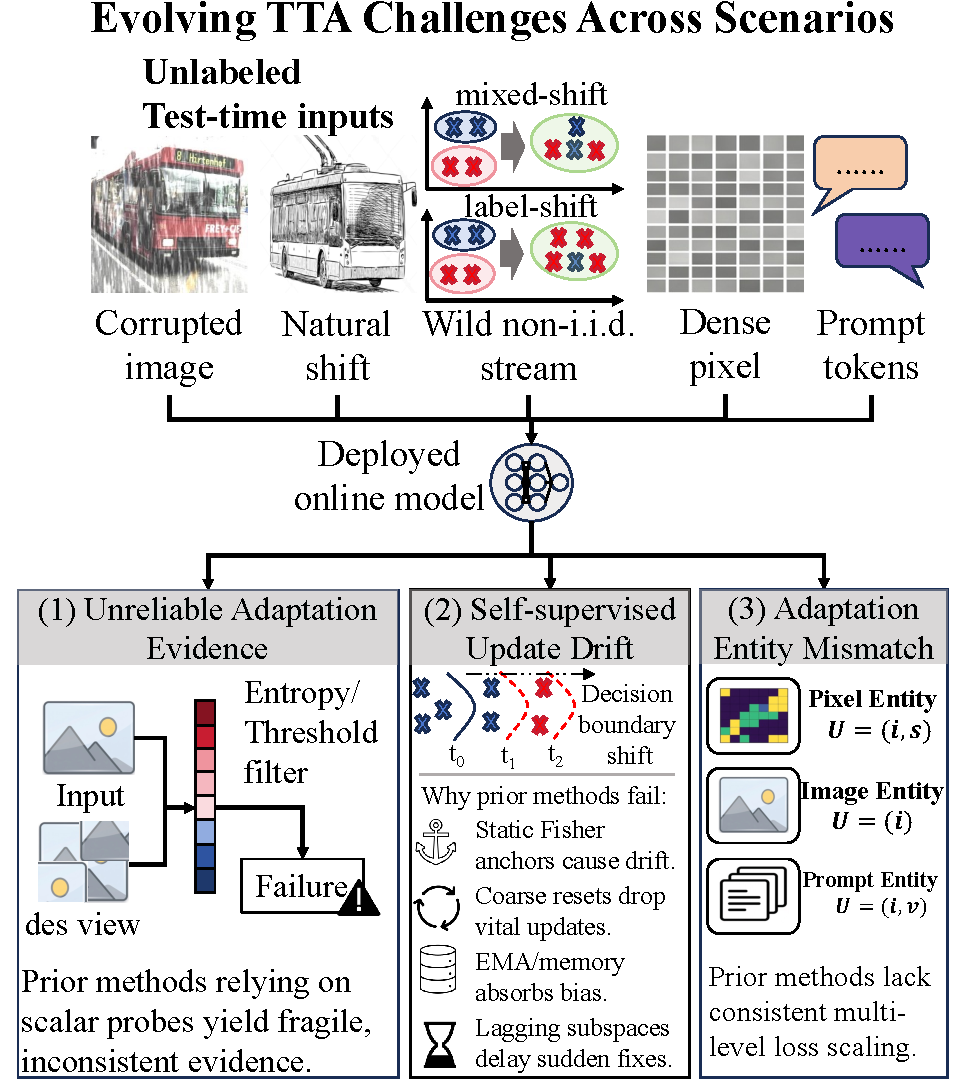
\includegraphics[width=\linewidth]{figures/fig1.pdf}
\caption{Overview of evolving test-time adaptation (TTA) challenges.}
\label{fig:tta_challenges}
\vspace{-10pt}
\end{wrapfigure}


The first problem is \emph{unreliable adaptation evidence}. \textsc{Tent} uses entropy as the adaptation signal, and later methods add filters, redundancy control, instability checks, or destructive probes~\citep{wang2021tent,niu2022eata,niu2023sar,lee2024deyo}. Low entropy alone, however, does not establish that a prediction is correct, and multiple target views can agree on the same mistake. Our hypothesis is that an entity is safer to update when semantics-preserving views corroborate the raw and source predictions and a structure-breaking view produces the expected sensitivity. Motivated by reliability analyses and VLM multi-view aggregation~\citep{press2024entropyenigma,farina2024zero}, \core{} operationalizes this hypothesis. We test it through selection ablations, same-role replacements, and signal diagnostics rather than treating confidence as sufficient evidence.

The second problem is \emph{drift after acceptance}. Because an online model supplies its own pseudo-targets, a selected sample can still move later predictions toward an unstable class. Fisher regularization, flat-minima recovery, teacher restoration, memory, gradient projection, and class debiasing provide different forms of drift control~\citep{niu2022eata,niu2023sar,wang2022cotta,yuan2023rotta,duan2025lifelong,ma2025adadem}. We hypothesize that an accepted update should have a stable reference appropriate to its model interface. \care{} uses source-relative clipping where direct source support is informative and class-centered support where online class geometry is the chosen reference. CORE-only and CORE+CARE ablations, together with continual and wild streams, test whether this anchoring reduces accumulated error.

The third problem is \emph{entity-count mismatch}. Classification selects images, segmentation selects pixels, and prompt adaptation selects view-conditioned predictions. Prior work studies class bias, dense alignment, hybrid segmentation adaptation, prompt tuning, caches, and forward-only search~\citep{ma2025adadem,jeon2025exploiting,de2025test,you2025test,park2025hybrid,shu2022tpt,ma2023swapprompt,feng2025diffusion,farina2024zero,karmanov2024tda,dai2025freetta,niu2024foa}. Our narrower hypothesis is that the loss scale should follow accepted prediction entities rather than all elements in the raw output tensor. \sane{} implements selected-entity normalization. The controlled selected-pixel versus total-pixel ablation tests this hypothesis directly for dense prediction; the prompt setting is reported as a separate task-specific instantiation rather than evidence of numerical equivalence.

Together, \core{}, \care{}, and \sane{} provide a common reliability vocabulary while retaining task-specific implementations. We evaluate ATLAS on CIFAR-100-C continual adaptation, ImageNet-C standard and continual adaptation, natural-shift ViT-B/16 recognition, wild ImageNet-C streams, Cityscapes$\rightarrow$ACDC segmentation, and episodic CLIP ViT-B/16 prompt adaptation. Across this protocol, \method{} reaches $68.8\%$ on CIFAR-100-C continual adaptation, $65.14\%$ on ViT-B/16 continual ImageNet-C, $59.16\%$ under batch-size-one wild streams, and $64.2\%$ OOD average accuracy for CLIP ViT-B/16 with CoOp initialization. The largest classification gains occur in continual and wild settings, where accepted errors can accumulate, while the dense-prediction ablation isolates the effect of selected-entity normalization.

The contributions are summarized as follows:
\begin{itemize}
\setlength{\itemsep}{2pt}
\setlength{\parsep}{0pt}
\setlength{\parskip}{0pt}
\setlength{\topsep}{3pt}
\setlength{\partopsep}{0pt}
\item We formulate TTA reliability as three testable factors: evidence selection, anchored updates, and normalization by selected prediction entities.
\item We instantiate these factors for image classification, semantic segmentation, and episodic prompt adaptation, and use component and normalization ablations to identify where the factors contribute.
\item We evaluate standard, continual, natural-shift, wild, dense-prediction, and prompt-adaptation settings, while reporting task-specific protocols, compatibility limits, efficiency, sensitivity, and observed failure modes.
\end{itemize}

\section{Related Work}

\subsection{Reliability signals for fully test-time adaptation}

Fully test-time adaptation often starts from entropy minimization. \textsc{Tent} updates normalization parameters by minimizing prediction entropy on unlabeled target data~\citep{wang2021tent}, and MEMO-style objectives add augmentation consistency~\citep{bartler2022memo}; related variants use contrastive objectives or parameter-free online updates~\citep{chen2022ctta,boudiaf2022potta}. Later work shows that low entropy alone is incomplete: \textsc{EATA} removes high-entropy and redundant samples while preserving source-important parameters~\citep{niu2022eata}, \textsc{SAR} combines reliable entropy with sharpness-aware recovery~\citep{niu2023sar}, \textsc{DeYO} uses destructive transformations to expose fragile confidence~\citep{lee2024deyo}, and \textsc{AdaDEM} analyzes reward collapse and easy-class bias~\citep{ma2025adadem}. \method{} follows this diagnosis, but \core{} shifts the reliability unit from a scalar sample score to a corroborated tensor entity checked by source, raw, photometric, structural, and destroy-view evidence.

\subsection{Drift control in continual and wild streams}

Continual TTA exposes cumulative drift because each accepted pseudo-supervised update changes the model that will supervise later inputs. \textsc{CoTTA} uses a mean teacher, augmentation-averaged pseudo-labels, and stochastic restoration~\citep{wang2022cotta}; \textsc{RoTTA} adds robust batch normalization and category-balanced memory~\citep{yuan2023rotta}; NOTE, DSS, and related teacher or memory methods stabilize online adaptation through replay, selection, or self-distillation~\citep{gong2022note,hong2024dss,song2023ecotta,doebler2023rmt}. PALM studies adaptive learning-rate control in continual TTA~\citep{maharana2025palm}. Lifelong Test-Time Adaptation constrains adaptation by projecting gradients into a tracked low-dimensional subspace~\citep{duan2025lifelong}, connecting continual TTA to intrinsic-dimension, low-dimensional training, and historical-solution averaging analyses~\citep{larsen2021intrinsic,li2022lowdim,li2023twa}. These results show that history and anchors matter in non-i.i.d. streams, but teachers, memories, normalization statistics, and gradient bases remain tied to specific stream and architecture assumptions. \care{} instead puts the anchor inside the loss for each accepted entity, using source-relative clipping or class-centered support rather than a separate stateful safeguard.

\subsection{Prompt and dense-prediction adaptation}

Vision-language and dense-prediction TTA broaden the adaptation entity beyond image-level classification. Prompt-only adaptation also draws on learned prompts, where CoOp, CoCoOp, ProDA, and MaPLe establish strong parameterizations for CLIP-style models~\citep{zhou2022learning,zhou2022conditional,khattak2022proda,khattak2023maple}. TPT adapts prompts through entropy minimization over selected augmented views~\citep{shu2022tpt}, while SwapPrompt, diffusion-enhanced TTA, DPCore, ZERO, TDA, FreeTTA, OT-VP, and FOA study prompt replacement, text-and-image augmentation, continual prompt memory, multi-view marginalization, caches, online distribution modeling, optimal transport, and forward-only VLM adaptation~\citep{ma2023swapprompt,feng2025diffusion,zhang2024dpcore,farina2024zero,karmanov2024tda,dai2025freetta,zhang2025otvp,niu2024foa}. Dense prediction introduces pixel-level imbalance, so segmentation adaptation studies domain properties, open-vocabulary optimization, correlation alignment, or hybrid adaptation~\citep{jeon2025exploiting,de2025test,you2025test,park2025hybrid}. These designs expose the same interface problem: images, pixels, and prompt views produce losses at different scales. \sane{} addresses it by normalizing \atlasloss{} over active selected entities, so update magnitude depends on accepted evidence rather than raw tensor count.

\section{Methodology}
\begin{figure*}[t]
\centering
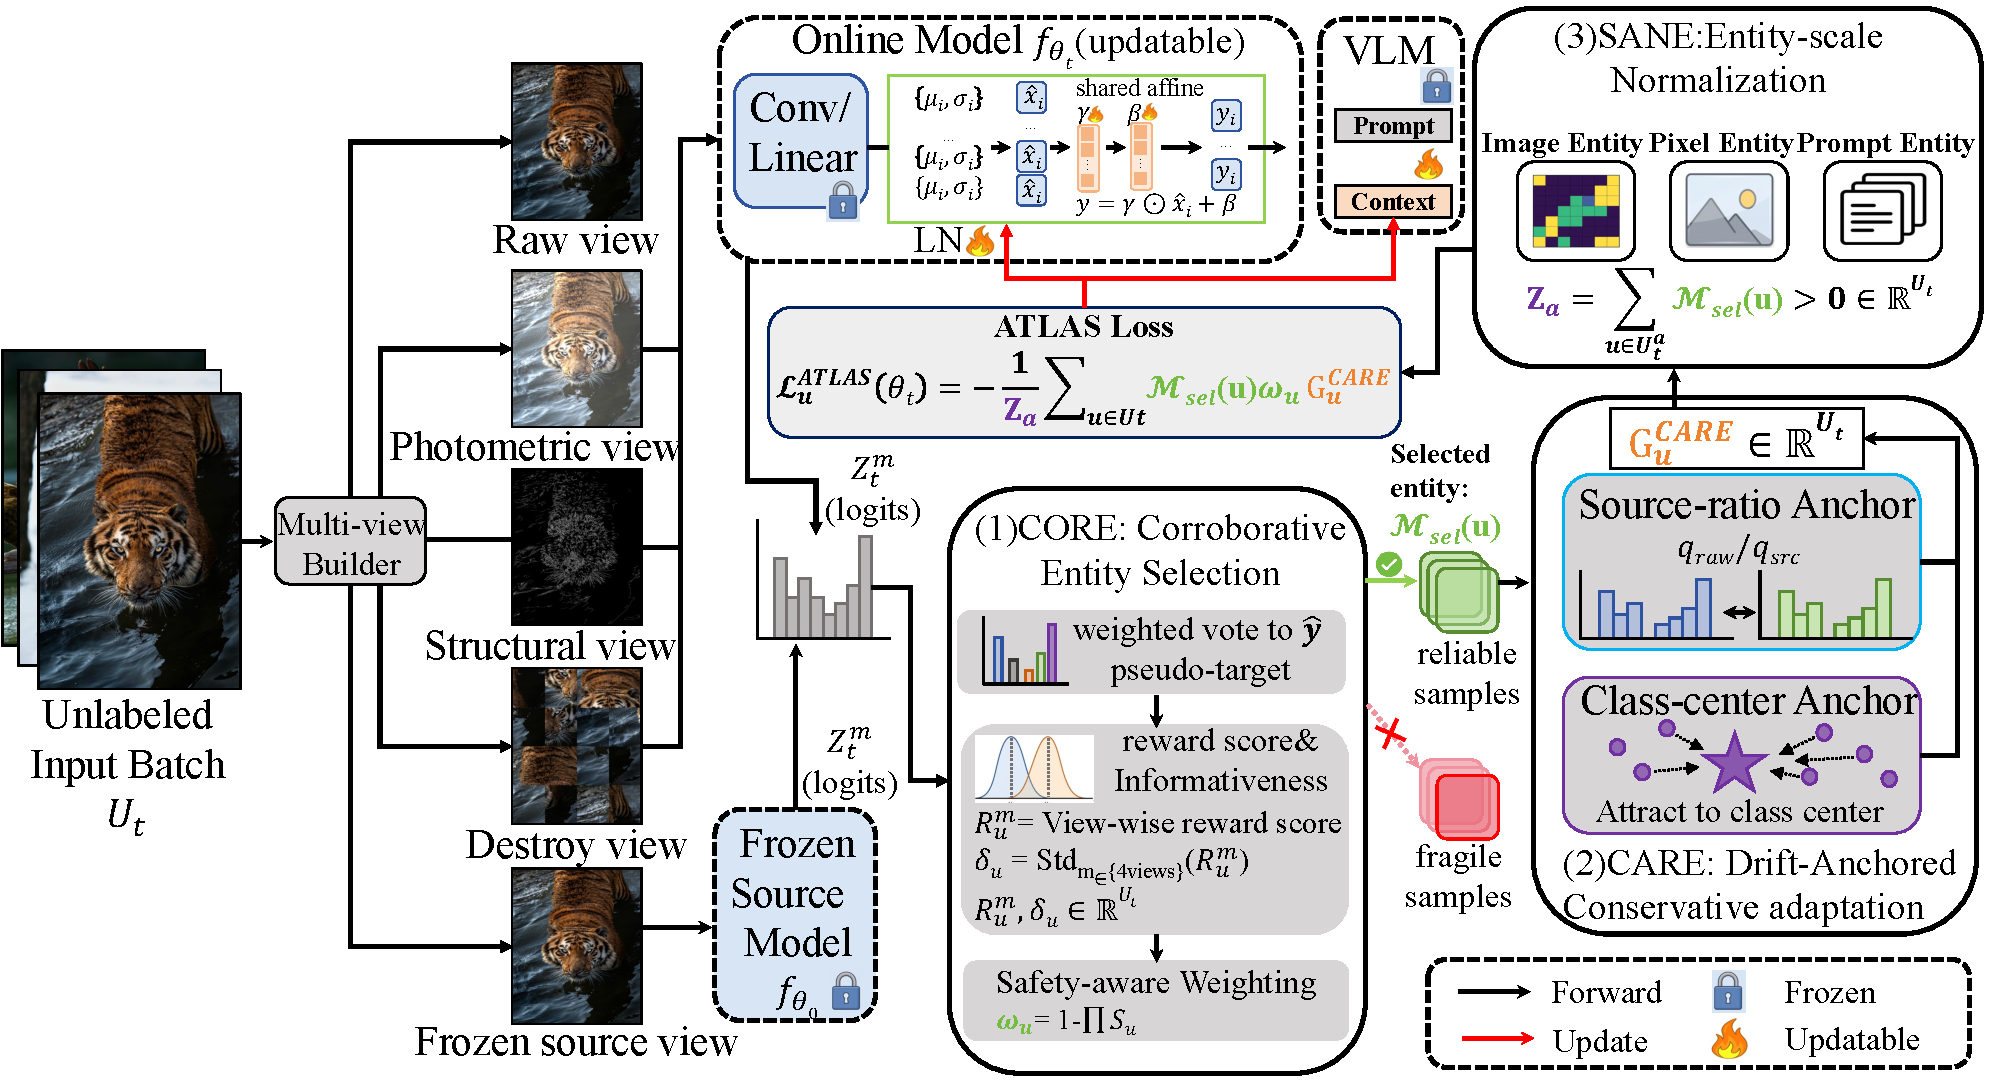
\includegraphics[width=1\linewidth]{figures/fig2-2.pdf}
\caption{Overview of the ATLAS framework. ATLAS builds multiple target views, selects safe and informative entities through CORE, constrains their updates with CARE, and normalizes the loss with SANE, updating only lightweight normalization or prompt parameters.}
\label{fig:atlas_pipeline}
\end{figure*}


\subsection{Problem setup}

Let $f(x;\theta)$ be a source model trained on a labeled source domain
$\mathcal{D}_s=\{(x_i,y_i)\}_{i=1}^{N}$ and deployed on an unlabeled target
stream $\mathcal{D}_t=\{x_t\}_{t=1}^{T}$. Fully test-time adaptation updates
the model online from target observations only~\citep{wang2021tent,niu2022eata}.
The classical entropy-minimization objective is
\begin{equation}
\mathcal{L}_{\mathrm{ent}}(x_t;\theta)
=
-\sum_{c=1}^{C}
p_{\theta}(y=c\mid x_t)\log p_{\theta}(y=c\mid x_t),
\qquad
p_{\theta}(\cdot\mid x_t)=\mathrm{softmax}(f(x_t;\theta)).
\label{eq:tent}
\end{equation}
Although this objective encourages confident predictions, it does not ask
whether confidence is corroborated, whether the update is anchored, or whether
losses are comparable across entity granularities.

This entity-centric view is close to slot-centric test-time adaptation, which studies decomposed object-centric representations rather than only whole-image predictions~\citep{prabhudesai2023test}.

ATLAS organizes its task-specific instantiations around primitive prediction entities. Let $B$ be the
target batch size, $\Omega_i$ the spatial lattice of image $i$, and $V$ the
number of prompt views. The entity set is
\begin{equation}
\begin{aligned}
\mathcal{U}_t^{\mathrm{img}}
&=\{\,i\,\}_{i=1}^{B},\\
\mathcal{U}_t^{\mathrm{pix}}
&=\{\,(i,s): i=1,\ldots,B,\; s\in\Omega_i\,\},\\
\mathcal{U}_t^{\mathrm{prm}}
&=\{\,(i,v): i=1,\ldots,B,\; v=1,\ldots,V\,\}.
\end{aligned}
\label{eq:entity_sets}
\end{equation}
Thus $u=i$ denotes an image-level prediction vector, $u=(i,s)$ a pixel-level
vector, and $u=(i,v)$ a prompt-view vector. The notation $\mathcal{U}_t^a$
denotes the active set, where
$a\in\{\mathrm{img},\mathrm{pix},\mathrm{prm}\}$.

For each entity, \method{} compares a frozen-source prediction, the current raw
prediction, a photometric view, a structural view, and a destroy view. Let
$z_u^m\in\mathbb{R}^{C}$ denote the pre-softmax logit vector for entity $u$
under view $m$, and let $p_u^m$ denote the corresponding class-probability
vector:
\begin{equation}
\mathcal{M}_{\mathrm{sup}}
=
\{\mathrm{src},\mathrm{raw},\mathrm{pho},\mathrm{str}\},
\qquad
\mathcal{M}_{\mathrm{all}}
=
\mathcal{M}_{\mathrm{sup}}\cup\{\mathrm{des}\},
\qquad
p_u^m=\mathrm{softmax}(z_u^m).
\label{eq:view_prob}
\end{equation}
The destroy view deliberately disrupts structure, e.g., by patch shuffling, to expose fragile confidence.


\subsection{Corroborative Entity Selection}

\core{} selects reliable entities from the view probabilities
$\{p_u^m\}_{m\in\mathcal{M}_{\mathrm{all}}}$. It first forms a pseudo-target by weighted voting:
\begin{equation}
\hat y_u
=
\arg\max_{c\in\mathcal{Y}}
\sum_{m\in\mathcal{M}_{\mathrm{sup}}}
\alpha_u^m
\mathbf{1}\!\left[
\arg\max_{j\in\mathcal{Y}}p_u^m(j)=c
\right],
\qquad
\alpha_u^m=\max_{c\in\mathcal{Y}}p_u^m(c)+\eta_m ,
\label{eq:vote}
\end{equation}
where $\eta_{\mathrm{src}}>0$ is a small source prior and $\eta_m=0$ for all $m\neq \mathrm{src}$.
The target-class probability is
\begin{equation}
q_u^m=p_u^m(\hat y_u),
\qquad
m\in\mathcal{M}_{\mathrm{all}}.
\label{eq:target_prob}
\end{equation}

Let
\begin{equation}
\bar H_u^m
=
-\frac{1}{\log C}
\sum_{c=1}^{C}p_u^m(c)\log p_u^m(c)
\label{eq:normalized_entropy}
\end{equation}
denote normalized entropy. We aggregate the four normalized evidence terms by
an equal mean, avoiding learned or benchmark-selected reward coefficients:
\begin{equation}
\begin{aligned}
R_u^m
=\frac{1}{4}\Big(&q_u^m+(1-\bar H_u^m)
+
\mathbf{1}\!\left[
\arg\max_c p_u^m(c)=\arg\max_c p_u^{\mathrm{src}}(c)
\right]
+
\mathbf{1}\!\left[
\arg\max_c p_u^m(c)=\hat y_u
\right]\Big).
\end{aligned}
\label{eq:reward}
\end{equation}
Its dispersion
\begin{equation}
\delta_u
=
\mathrm{Std}_{m\in\{\mathrm{raw},\mathrm{pho},\mathrm{str},\mathrm{des}\}}
(R_u^m)
\label{eq:dispersion}
\end{equation}
measures whether the views provide differential evidence.

The safety score combines entropy, source disagreement, view inconsistency, and insufficient destroy-view sensitivity:
\begin{equation}
s_u
=
\lambda_e\bar H_u^{\mathrm{raw}}
+\lambda_a\Delta_u^{\mathrm{anchor}}
+\lambda_v\Delta_u^{\mathrm{view}}
+\lambda_d[\rho_d-\Delta_u^{\mathrm{des}}]_+,
\label{eq:safety_score}
\end{equation}
with
\begin{equation}
\begin{aligned}
\Delta_u^{\mathrm{anchor}}
&=
\mathbf{1}\!\left[
\arg\max_c p_u^{\mathrm{raw}}(c)
\ne
\arg\max_c p_u^{\mathrm{src}}(c)
\right],\\
\Delta_u^{\mathrm{view}}
&=
1-\frac{1}{2}
\sum_{m\in\{\mathrm{pho},\mathrm{str}\}}
\mathbf{1}\!\left[
\arg\max_c p_u^m(c)
=
\arg\max_c p_u^{\mathrm{raw}}(c)
\right],\\
\Delta_u^{\mathrm{des}}
&=
[q_u^{\mathrm{raw}}-q_u^{\mathrm{des}}]_+ .
\end{aligned}
\label{eq:safety_terms}
\end{equation}
Here $\rho_d>0$ is the minimum destroy-view confidence drop required before an entity is treated as structurally supported.
The soft safety weight is
\begin{equation}
\omega_u
=
1-\Pi(s_u;m_{\mathrm{safe}},m_{\mathrm{hard}}),
\qquad
\Pi(s;m_{\mathrm{safe}},m_{\mathrm{hard}})
=
\begin{cases}
0, & s\le m_{\mathrm{safe}},\\[2pt]
\dfrac{s-m_{\mathrm{safe}}}{m_{\mathrm{hard}}-m_{\mathrm{safe}}},
& m_{\mathrm{safe}}<s<m_{\mathrm{hard}},\\[8pt]
1, & s\ge m_{\mathrm{hard}}.
\end{cases}
\label{eq:safe}
\end{equation}
For the Core variant, the normalized evidence terms define a reliability score
$e_u$ (their available-term mean), and the final selection mask is
\begin{equation}
\mathcal{M}_{\mathrm{sel}}(u)
=
\mathbf{1}\!\left[e_u\ge Q_q(\{e_v:v\in\mathcal U_t\})\right],
\label{eq:selected}
\end{equation}
where $Q_q$ is computed only from the current unlabeled adaptation entities and
$q=0.5$ throughout. Thus the Core gate transfers by score order rather than an
absolute entropy, PLPD, dispersion, or safety threshold. Full retains the
branch refinements audited in the supplement and is reported separately.

\subsection{Drift-Anchored Conservative Adaptation}

\care{} anchors the update of selected entities. When source support is reliable, it uses the raw-view advantage
\begin{equation}
A_u
=
\frac{
R_u^{\mathrm{raw}}
-
\frac{1}{4}
\sum_{m\in\{\mathrm{raw},\mathrm{pho},\mathrm{str},\mathrm{des}\}}R_u^m
}
{\delta_u+\varepsilon}
\label{eq:advantage}
\end{equation}
and the entity-level source-relative ratio
\begin{equation}
r_u
=
\frac{q_u^{\mathrm{raw}}+\varepsilon}
{q_u^{\mathrm{src}}+\varepsilon}.
\label{eq:ratio}
\end{equation}
The conservative clipped surrogate is
\begin{equation}
\phi(r_u,A_u)
=
\min\!\left(
r_uA_u,\,
\operatorname{clip}(r_u,1-\epsilon_{\mathrm{low}},1+\epsilon_{\mathrm{high}})A_u
\right).
\label{eq:clip}
\end{equation}
The signed advantage and two-sided PPO surrogate prevent improvement beyond the
upper clip for $A_u>0$ and prevent deterioration beyond the lower clip for
$A_u<0$. Eq.~\ref{eq:atlas_loss} minimizes its negative normalized form.

When class structure is more reliable than direct source matching, \care{} uses a class-centered anchor. For pseudo-class $\hat y_u$ with online
center $c_{\hat y_u}^t\in\mathbb{R}^{C}$,
\begin{equation}
\ell_u^{\mathrm{center}}
=
\frac{(p_u^{\mathrm{raw}}-\operatorname{stopgrad}(c_{\hat y_u}^{t}))^\top
z_u^{\mathrm{raw}}}{g_u},
\quad
g_u=\left\|\bigl(z_u^{\mathrm{raw}}+T_u+1\bigr)\odot
p_u^{\mathrm{raw}}\right\|_1,
\quad
T_u=-\sum_c p_u^{\mathrm{raw}}(c)z_u^{\mathrm{raw}}(c).
\label{eq:centered}
\end{equation}
The stopped-gradient center is the conservative reference. The scale $g_u$ is
also detached; a finite-difference test verifies that a descent step reduces
$D_{\mathrm{KL}}(c_{\hat y_u}^{t}\|p_u^{\mathrm{raw}})$. The entity-level \care{} support is
\begin{equation}
G_{\mathrm{u}}^{CARE}
=
\begin{cases}
\phi(r_u,A_u),
& \text{source-relative anchor},\\[2pt]
-\ell_u^{\mathrm{center}},
& \text{class-centered anchor},\\[2pt]
0,
& \text{otherwise}.
\end{cases}
\label{eq:anc_entity}
\end{equation}
Equivalently, the per-entity loss is $\ell_{\mathrm{u}}^{CARE}=-G_{\mathrm{u}}^{CARE}$ before entity-scale normalization.

\subsection{Entity-Scale Normalization}

\sane{} normalizes by the number of selected primitive prediction entities.
% The uppercase symbol $Z_a$ denotes this entity-scale normalizer, which
% is distinct from the lowercase logits $z_u^m$ defined above.
For the three scenarios,
\begin{equation}
Z_{\mathrm{img}}
=
\sum_{i=1}^{B}\mathcal{M}_{\mathrm{sel}}(i),
\qquad
Z_{\mathrm{pix}}
=
\sum_{i=1}^{B}\sum_{s\in\Omega_i}\mathcal{M}_{\mathrm{sel}}(i,s),
\qquad
Z_{\mathrm{prm}}
=
\sum_{i=1}^{B}\sum_{v=1}^{V}\mathcal{M}_{\mathrm{sel}}(i,v).
\label{eq:sane_three_cases}
\end{equation}
% \begin{equation}
% \begin{aligned}
% Z_{\mathrm{img}}
% &=
% \sum_{i=1}^{B}
% \mathcal{M}_{\mathrm{sel}}(i),\\
% Z_{\mathrm{pix}}
% &=
% \sum_{i=1}^{B}
% \sum_{s\in\Omega_i}
% \mathcal{M}_{\mathrm{sel}}(i,s),\\
% Z_{\mathrm{prm}}
% &=
% \sum_{i=1}^{B}
% \sum_{v=1}^{V}
% \mathcal{M}_{\mathrm{sel}}(i,v).
% \end{aligned}
% \label{eq:sane_three_cases}
% \end{equation}
Equivalently,
\begin{equation}
Z_a
=
\sum_{u\in\mathcal{U}_t^a}
\mathcal{M}_{\mathrm{sel}}(u),
\qquad
a\in\{\mathrm{img},\mathrm{pix},\mathrm{prm}\}.
\label{eq:sane_unified}
\end{equation}

If $Z_a=0$, the adaptation step is skipped. Evidence weights in the numerator
are detached, while the denominator is the integer selected-entity count rather
than weighted mass or total output size. In the denominator, ATLAS uses a small
constant $\varepsilon_Z>0$ for numerical stability.

\subsection{The \atlasloss{}}

\core{}, \care{}, and \sane{} yield the final objective
\begin{equation}
\mathcal{L}_{\text{\textsc{ATLAS}}}^{a}(\theta_t)
=
-\frac{1}{Z_a+\varepsilon_Z}
\sum_{u\in\mathcal{U}_t^a}
\underbrace{
\mathcal{M}_{\mathrm{sel}}(u)\omega_u
}_{\text{\core{} selection}}
\underbrace{
G_{\mathrm{u}}^{CARE}
}_{\text{\care{} anchoring}},
\qquad
a\in\{\mathrm{img},\mathrm{pix},\mathrm{prm}\}.
\label{eq:atlas_loss}
\end{equation}
Thus \core{} selects reliable entities, \care{} anchors their update direction, and \sane{} makes the loss comparable across image-, pixel-, and prompt-view adaptation. Appendix~\ref{app:atlas_executable} starts with a compact principle-versus-instantiation table and then records the online update used in the artifact, including the scenario-specific gate $\gamma_u$, the exposed paper-level hyperparameters, the EMA class-center update, and the branch-level choice between the two CARE anchors.

% \subsection{Scenario instantiations}

% \paragraph{Classification.}
% The active set is $\mathcal{U}_t^{\mathrm{img}}$, where each entity $u=i$ is one
% image-level prediction vector. The normalizer is $Z_{\mathrm{img}}$.

% \paragraph{Segmentation.}
% The active set is $\mathcal{U}_t^{\mathrm{pix}}$, where each entity $u=(i,s)$ is
% one pixel-level prediction vector at location $s$. The normalizer is
% $Z_{\mathrm{pix}}$.

% \paragraph{Vision-language adaptation.}
% The active set is $\mathcal{U}_t^{\mathrm{prm}}$, where each entity $u=(i,v)$ is
% one prompt-view prediction vector. The normalizer is $Z_{\mathrm{prm}}$.

\begin{table*}[hbtp]
\centering
\footnotesize
\setlength{\tabcolsep}{3.0pt}
\renewcommand{\arraystretch}{1.09}
\caption{CIFAR-100-C under continual adaptation over the 15-corruption stream, with all methods using the same ResNeXt-29 backbone. Results are reported as mean $\pm$ std over three random orders. Best in \textbf{bold}; second-best \underline{underlined}.}
\label{tab:l1a}
\resizebox{\textwidth}{!}{%
\begin{tabular}{lccccccccccccccc!{\color{black!35}\vrule width 0.45pt}c}
\toprule
Method & Bright. & Contr. & Defoc. & Elastic & Fog & Frost & Gauss. & Glass & Impulse & JPEG & Motion & Pixel. & Shot & Snow & Zoom & \avg \\
\midrule
Source & \res{70.5}{0.0} & \res{44.9}{0.0} & \res{70.7}{0.0} & \res{62.8}{0.0} & \res{49.7}{0.0} & \res{54.2}{0.0} & \res{27.0}{0.0} & \res{45.9}{0.0} & \res{60.6}{0.0} & \res{58.8}{0.0} & \res{69.2}{0.0} & \res{25.3}{0.0} & \res{32.0}{0.0} & \res{60.5}{0.0} & \res{71.2}{0.0} & \res{53.6}{0.0} \\
Tent (ICLR'21) & \res{74.5}{0.3} & \res{67.4}{3.7} & \res{71.3}{2.6} & \res{66.0}{1.2} & \res{62.8}{1.0} & \res{64.9}{1.5} & \res{62.2}{1.3} & \res{62.4}{1.2} & \res{58.9}{0.6} & \res{60.2}{2.4} & \res{68.6}{2.7} & \res{68.2}{2.8} & \res{63.7}{2.8} & \res{65.2}{2.7} & \res{68.4}{0.8} & \res{65.6}{0.4} \\
EATA (ICML'22) & \res{74.0}{0.3} & \res{70.2}{0.5} & \res{72.5}{0.6} & \res{66.7}{0.3} & \res{63.1}{1.0} & \res{67.7}{0.7} & \res{62.3}{0.2} & \res{62.4}{0.1} & \res{61.9}{0.2} & \res{60.7}{0.4} & \res{70.1}{0.6} & \res{69.8}{0.4} & \res{64.7}{0.3} & \res{67.1}{0.7} & \res{72.5}{0.5} & \res{67.1}{0.0} \\
SAR (ICLR'23) & \res{73.3}{0.1} & \res{69.7}{0.0} & \res{72.4}{0.0} & \res{66.1}{1.2} & \res{61.7}{0.7} & \res{66.5}{0.2} & \res{61.2}{0.9} & \res{61.1}{1.4} & \best{63.3}{1.0} & \res{61.0}{1.1} & \res{70.6}{0.1} & \res{68.1}{0.0} & \res{62.9}{1.3} & \res{68.0}{0.1} & \res{71.9}{0.1} & \res{66.5}{0.1} \\
CoTTA (CVPR'22) & \res{72.0}{0.0} & \res{65.9}{0.5} & \res{69.6}{0.3} & \res{65.7}{0.3} & \res{58.7}{0.2} & \res{66.8}{0.1} & \res{62.4}{0.3} & \ulres{62.9}{0.2} & \res{61.8}{0.0} & \best{63.6}{0.9} & \res{69.0}{0.4} & \res{69.8}{0.1} & \res{63.6}{0.6} & \res{65.4}{0.2} & \res{69.7}{0.1} & \res{65.8}{0.1} \\
LCoTTA (NeurIPS'25) & \res{73.9}{0.3} & \res{70.4}{0.8} & \res{72.6}{0.7} & \res{66.7}{0.3} & \res{62.6}{1.1} & \res{67.9}{0.6} & \res{62.4}{0.2} & \res{62.6}{0.6} & \res{61.3}{1.0} & \res{60.7}{0.3} & \res{70.3}{0.4} & \res{69.9}{0.8} & \res{64.6}{0.7} & \res{67.1}{0.6} & \res{72.8}{0.2} & \res{67.0}{0.0} \\
AdaDEM (NeurIPS'25) & \res{73.9}{0.4} & \res{71.3}{0.7} & \res{74.0}{0.6} & \res{66.7}{0.8} & \res{61.4}{0.3} & \res{68.2}{0.6} & \res{61.3}{1.0} & \res{61.6}{0.3} & \res{62.0}{0.1} & \res{59.9}{1.1} & \ulres{72.0}{0.5} & \res{69.8}{1.1} & \res{63.1}{1.6} & \res{67.5}{0.3} & \best{74.6}{0.0} & \res{67.1}{0.0} \\
SURGEON (CVPR'25) & \ulres{74.7}{1.4} & \res{65.8}{6.3} & \res{68.3}{4.5} & \res{65.9}{1.9} & \res{62.6}{2.7} & \res{64.7}{3.5} & \ulres{63.8}{1.6} & \res{62.9}{1.0} & \res{57.4}{1.1} & \ulres{63.5}{1.4} & \res{66.2}{3.9} & \res{68.8}{1.9} & \ulres{65.6}{1.0} & \res{66.0}{1.2} & \res{65.5}{2.7} & \res{65.4}{1.3} \\
DeYO (ICLR'24) & \best{74.8}{0.1} & \ulres{72.1}{0.4} & \ulres{74.2}{0.4} & \ulres{67.7}{0.2} & \ulres{63.6}{0.6} & \ulres{68.7}{0.1} & \res{62.8}{0.2} & \res{62.4}{0.2} & \res{62.4}{0.2} & \res{62.3}{0.6} & \res{71.8}{0.3} & \ulres{70.7}{0.2} & \res{64.7}{0.3} & \ulres{68.1}{0.2} & \res{74.0}{0.2} & \ulres{68.0}{0.1} \\
RoTTA (CVPR'23) & \res{71.6}{0.9} & \res{60.6}{12.8} & \res{72.5}{2.1} & \res{66.2}{1.1} & \res{61.7}{0.3} & \res{68.5}{0.8} & \res{58.6}{3.0} & \res{59.4}{2.0} & \res{59.2}{0.3} & \res{57.0}{5.0} & \res{71.1}{1.4} & \res{67.1}{4.0} & \res{59.4}{4.0} & \res{67.4}{1.3} & \ulres{74.2}{0.5} & \res{65.0}{0.1} \\
\midrule
\rowcolor{gray!10}
\textbf{\method{}} & \res{74.6}{0.6} & \best{72.8}{0.3} & \best{74.4}{0.6} & \best{68.5}{0.1} & \best{64.7}{0.6} & \best{70.2}{0.5} & \best{64.3}{0.2} & \best{64.9}{0.1} & \ulres{63.2}{0.3} & \res{61.8}{1.1} & \best{72.2}{0.4} & \best{71.4}{0.5} & \best{66.2}{0.5} & \best{69.1}{0.3} & \res{74.0}{0.0} & \best{68.8}{0.2} \\
\bottomrule
\end{tabular}}
\end{table*}

\section{Experiments and Results}

\subsection{Experimental setup and five-level protocol}

The evaluation follows a five-level protocol. Level 1 studies CIFAR-100-C and ImageNet-C under standard TTA, where the model resets between corruptions, and continual TTA, where one model processes the full stream without gradient reset~\citep{wang2021tent,wang2022cotta}. Both use the $15$ ImageNet-C corruption types at severity $5$~\citep{hendrycks2019imagenetc}. Level 2 tests natural shifts on ImageNet-A, ImageNet-R, ImageNet-V2, and ImageNet-Sketch with ViT-B/16~\citep{dosovitskiy2021vit,hendrycks2021imageneta,hendrycks2021manyfaces,recht2021imagenetv2}. Level 3 evaluates wild non-i.i.d. streams under label shift, mixed shifts, and batch-size-one inference, following WILDS~\citep{koh2021wilds}. Level 4 studies Cityscapes$\rightarrow$ACDC segmentation with SegFormer-B5~\citep{cordts2016cityscapes,sakaridis2021acdc,xie2021segformer}. Level 5 studies prompt-only adaptation for CLIP ViT-B/16~\citep{radford2021clip}. Classification and VLM experiments report top-1 accuracy; segmentation reports online error and mIoU. Means $\pm$ standard deviations are reported when available. Standard corruption runs use three random seeds; continual runs use three random corruption orders. The protocol isolates unreliable evidence, online drift, and entity-scale mismatch.

\subsection{Level 1: Synthetic corruptions}


\begin{wraptable}{r}{0.60\columnwidth}
\vspace{-1.2\baselineskip}
\centering
\normalsize
\setlength{\tabcolsep}{3pt}
\renewcommand{\arraystretch}{1.05}
\caption{\textbf{ImageNet-C under standard and continual adaptation.}
Standard columns report mean $\pm$ std across three random seeds; continual columns report mean $\pm$ std across three random corruption orders. Unsupported entries are excluded from best-baseline margins; collapse entries are raw official-scope reproductions and are not used as the primary comparison. Best in \textbf{bold}; second-best \underline{underlined}.}
\label{tab:l2}
\resizebox{\linewidth}{!}{%
\begin{tabular}{@{}lcccc@{}}
\toprule
& \multicolumn{2}{c}{ResNet-50-GN} & \multicolumn{2}{c}{ViT-B/16} \\
\cmidrule(lr){2-3}\cmidrule(lr){4-5}
Method & Standard & Continual & Standard & Continual \\
\midrule
Source & \res{31.44}{0.00} & \res{31.44}{0.00} & \res{39.83}{0.00} & \res{39.83}{0.00} \\
Tent (ICLR'21) & \res{32.02}{0.00} & \res{21.84}{1.38} & \res{54.62}{0.03} & \res{49.02}{0.14} \\
EATA (ICML'22) & \res{41.89}{0.02} & \ulres{34.82}{0.57} & \res{58.25}{1.09} & \res{18.04}{8.68} \\
SAR (ICLR'23) & \res{35.84}{0.00} & \res{32.30}{8.20} & \res{54.57}{0.03} & \res{55.88}{0.58} \\
CoTTA (CVPR'22) & \res{31.49}{0.00} & \res{31.44}{0.03} & \res{40.25}{0.00} & \res{42.10}{0.09} \\
Lifelong TTA (NeurIPS'25) & \res{40.36}{0.00} & \res{34.02}{0.79} & \ulres{60.18}{0.10} & \res{36.73}{0.20} \\
AdaDEM (NeurIPS'25) & \res{32.21}{0.00} & \res{30.72}{0.29} & \res{58.94}{1.83} & \ulres{64.11}{0.43} \\
FOA (ICML'24) & \multicolumn{1}{c}{\pending} & \multicolumn{1}{c}{\pending} & \res{48.98}{0.18} & \res{48.56}{0.34} \\
DeYO (ICLR'24) & \ulres{43.79}{0.01} & \res{23.98}{13.91} & \res{60.00}{0.59} & \res{56.52}{0.40} \\
\midrule
\rowcolor{gray!8}
\textbf{\method{}} & \best{48.40}{0.07} & \best{45.84}{0.08} & \best{60.21}{0.03} & \best{65.14}{0.05} \\
\bottomrule
\end{tabular}}
\vspace{-0.8\baselineskip}
\end{wraptable}

% \begin{table*}[t]
% \centering
% \small
% \setlength{\tabcolsep}{6pt}
% \renewcommand{\arraystretch}{1.08}
% \caption{\textbf{ImageNet-C under standard and continual adaptation.}
% Results are reported as mean \(\pm\) std across three random orders. The best result in each column is highlighted in \textbf{bold}, and the second-best is \underline{underlined}.}
% \label{tab:l2}
% \begin{tabular}{@{}lcccc@{}}
% \toprule
% & \multicolumn{2}{c}{ResNet-50-GN} & \multicolumn{2}{c}{ViT-B/16} \\
% \cmidrule(lr){2-3}\cmidrule(lr){4-5}
% Method & Standard & Continual & Standard & Continual \\
% \midrule
% Source & \res{31.44}{0.00} & \res{31.44}{0.00} & \res{39.83}{0.00} & \res{39.83}{0.00} \\
% Tent (ICLR'21) & \res{32.02}{0.00} & \res{21.84}{1.38} & \res{54.62}{0.03} & \res{49.02}{13.95} \\
% EATA (ICML'22) & \res{41.89}{0.02} & \ulres{34.82}{0.57} & \res{58.25}{1.09} & \res{18.04}{8.68} \\
% SAR (ICLR'23) & \res{35.84}{0.00} & \res{32.30}{8.20} & \res{54.57}{0.03} & \res{55.88}{0.58} \\
% CoTTA (CVPR'22) & \res{31.49}{0.00} & \res{31.44}{0.03} & \res{40.25}{0.00} & \res{42.10}{0.09} \\
% Lifelong TTA (NeurIPS'25) & \res{40.36}{0.00} & \res{34.02}{0.79} & \ulres{60.18}{0.10} & \res{36.73}{0.20} \\
% AdaDEM (NeurIPS'25) & \res{32.21}{0.00} & \res{30.72}{0.29} & \res{58.94}{1.83} & \ulres{64.11}{0.43} \\
% SURGEON (CVPR'25) & \res{0.18}{0.01} & \res{0.13}{0.01} & \res{5.03}{0.57} & \res{3.17}{2.05} \\
% FOA (ICML'24) & \multicolumn{1}{c}{\pending} & \multicolumn{1}{c}{\pending} & \res{48.98}{0.18} & \res{48.56}{0.34} \\
% DeYO (ICLR'24) & \ulres{43.79}{0.01} & \res{23.98}{13.91} & \res{60.00}{0.59} & \res{56.52}{0.40} \\
% \midrule
% \rowcolor{gray!8}
% \textbf{\method{}} & \best{48.40}{0.07} & \best{45.84}{0.08} & \best{60.21}{0.03} & \best{65.14}{0.05} \\
% \bottomrule
% \end{tabular}
% \end{table*}
% % \begin{table}[htbp]
% % \centering
% % \small
% % \caption{ImageNet-C under standard and continual adaptation. Entries marked with - denote absent or invalid reproductions in the current artifact set.}
% % \label{tab:l2}
% % \resizebox{\textwidth}{!}{%
% % \begin{tabular}{llcc|llcc}
% % \toprule
% % Backbone & Method & Standard & Continual & Backbone & Method & Standard & Continual \\
% % \midrule
% % \multirow{12}{*}{ResNet-50-GN}
% % & Source & 31.44 & 31.44
% % & \multirow{12}{*}{ViT-B/16}
% % & Source & 39.83 & 39.83 \\
% % & Tent (ICLR'21) & 32.02 & 21.84
% % && Tent (ICLR'21) & 54.62 & 49.02 \\
% % & EATA (ICML'22) & 41.89 & 34.82
% % && EATA (ICML'22) & 58.25 & 18.04 \\
% % & SAR (ICLR'23) & 35.84 & 32.30
% % && SAR (ICLR'23) & 54.57 & 55.88 \\
% % & CoTTA (CVPR'22) & 31.49 & 31.44
% % && CoTTA (CVPR'22) & 40.25 & 42.10 \\
% % & Lifelong TTA (NeurIPS'25) & 40.36 & 34.02
% % && Lifelong TTA (NeurIPS'25) & 60.18 & 36.73 \\
% % & AdaDEM (NeurIPS'25) & 32.21 & 30.72
% % && AdaDEM (NeurIPS'25) & 58.94 & 64.11 \\
% % & SURGEON (CVPR'25) & 0.18 & 0.13
% % && SURGEON (CVPR'25) & 5.03 & 3.17 \\
% % & FOA (ICML'24) & - & -
% % && FOA (ICML'24) & 48.98 & 48.56 \\
% % & DeYO (ICLR'24) & 43.79 & 23.98
% % && DeYO (ICLR'24) & 60.00 & 56.52 \\
% % % & RoTTA (CVPR'23) & 31.44 & 31.44
% % % && RoTTA (CVPR'23) & 39.83 & 39.83 \\
% % & \method{} & 31.68 & 31.95
% % && \method{} & 41.41 & 42.43 \\
% % \bottomrule
% % \end{tabular}}
% % \end{table}


Synthetic corruptions test whether a TTA method can reject unsafe confidence while still adapting to degraded inputs. On CIFAR-100-C continual adaptation, Table~\ref{tab:l1a} shows \method{} at $68.8\pm0.2$, beating DeYO by $0.8$ points and EATA/AdaDEM by $1.7$. It is best on $11$ of $15$ corruptions, covering both photometric and structure-changing cases. Appendix~\ref{app:additional_cifar} reports the standard CIFAR-100-C protocol, where \method{} reaches $69.1\pm0.0$, $0.4$ points above SURGEON become new best method.

ImageNet-C exposes the same reliability issue across backbones. In Table~\ref{tab:l2}, \method{} reaches $48.40\pm0.07$ on ResNet-50-GN standard adaptation and $45.84\pm0.08$ on ResNet-50-GN continual adaptation, improving over the strongest baselines by $4.61$ and $11.02$ points. On ViT-B/16, it reaches $60.21\pm0.03$ in the standard setting and $65.14\pm0.05$ in the continual setting, improving over the best baselines by $0.03$ and $1.03$ points. The small ViT standard margin and larger continual margins suggest that \method{} helps most when stream order and drift matter.

\subsection{Level 2: Natural distribution shifts}
\begin{table*}[b]
\centering
\begin{minipage}[t]{0.59\textwidth}
\centering
\footnotesize
\setlength{\tabcolsep}{3.5pt}
\captionof{table}{Natural-shift OOD performance on ViT-B/16. Collapse entries are raw official-scope reproductions and are not used as the primary comparison. Best in bold; second-best underlined.}
\label{tab:l3}

\adjustbox{max width=\linewidth}{%
\begin{tabular}{lccccc}
\toprule
Method & IN-A & IN-R & IN-V2 & IN-Sketch & Avg. \\
\midrule
Source   & \res{15.61}{0.00} & \res{35.14}{0.00} & \res{69.42}{0.00} & \res{27.85}{0.00} & \res{37.01}{0.00} \\
Tent     & \res{17.95}{0.02} & \res{38.23}{0.05} & \ulres{69.77}{0.17} & \res{33.72}{2.09} & \res{39.92}{0.58} \\
EATA     & \res{17.04}{0.02} & \res{35.75}{0.80} & \res{69.62}{0.07} & \res{38.99}{0.28} & \res{40.35}{0.21} \\
SAR      & \res{17.78}{0.06} & \res{36.61}{0.05} & \res{69.56}{0.07} & \res{33.91}{0.06} & \res{39.47}{0.02} \\
CoTTA    & \res{15.61}{0.00} & \res{35.17}{0.00} & \res{69.44}{0.00} & \res{27.88}{0.00} & \res{37.02}{0.00} \\
LCoTTA   & \res{17.02}{0.94} & \res{34.34}{0.41} & \res{69.36}{0.02} & \res{37.96}{0.96} & \res{39.67}{0.14} \\
AdaDEM   & \ulres{18.59}{1.64} & \res{44.39}{0.23} & \res{68.14}{0.17} & \res{4.96}{0.32} & \res{34.02}{0.37} \\
FOA      & \res{15.49}{0.10} & \res{0.11}{0.00} & \res{69.63}{0.04} & \res{28.88}{0.04} & \res{28.53}{0.03} \\
DeYO     & \res{18.46}{0.80} & \ulres{44.52}{0.13} & \res{69.67}{0.17} & \ulres{40.19}{0.05} & \ulres{43.21}{0.22} \\
\rowcolor{gray!10}
\method{} & \best{21.74}{1.06} & \best{45.25}{0.29} & \best{70.50}{0.16} & \best{41.19}{0.20} & \best{44.67}{0.36} \\
\bottomrule
\end{tabular}
}
\end{minipage}
\hfill
\begin{minipage}[t]{0.39\textwidth}
\centering
\footnotesize
\setlength{\tabcolsep}{4pt}
\captionof{table}{Wild ImageNet-C on ViT-B/16 under label shift, mixed shifts, and BS=1. Unsupported entries are excluded from best-baseline margins.}
% ; collapse entries are shown only as raw official-scope reproductions.}
\label{tab:l4}

\adjustbox{max width=\linewidth}{%
\begin{tabular}{lccc}
\toprule
Method & Label shift & Mixed shifts & BS=1 \\
\midrule
Source & \res{39.75}{0.00} & \res{39.83}{0.00} & \res{39.83}{0.00} \\
Tent & \res{50.33}{0.16} & \res{58.80}{0.16} & \res{5.38}{0.04} \\
EATA & \res{33.89}{0.23} & \res{60.91}{0.23} & \res{2.61}{0.20} \\
SAR & \res{56.52}{0.15} & \res{53.60}{0.15} & \ulres{55.82}{0.47} \\
CoTTA & \res{41.84}{0.01} & \res{42.60}{0.01} & \res{44.35}{0.02} \\
LCoTTA & \res{45.33}{3.34} & \ulres{61.01}{3.34} & \res{32.08}{22.63} \\
AdaDEM & \res{6.01}{0.24} & \res{60.65}{0.24} & \res{0.18}{0.10} \\
% SURGEON & - & - & - \\
FOA & \res{49.24}{0.04} & \res{49.69}{0.04} & \res{0.64}{0.04} \\
DeYO & \ulres{56.66}{0.28} & \res{53.57}{0.28} & \res{5.51}{0.28} \\
% RoTTA & - & - & - \\
\rowcolor{gray!10}
\method{} & \best{57.47}{0.41} & \best{61.67}{0.41} & \best{59.16}{0.41} \\
\bottomrule
\end{tabular}%
}
\end{minipage}
\end{table*}


Natural shifts test transfer to semantic changes rather than synthetic corruptions. Table~\ref{tab:l3} reports ViT-B/16 results on ImageNet-A, ImageNet-R, ImageNet-V2, and ImageNet-Sketch. \method{} reaches $44.67\pm0.36$ average accuracy, $1.46$ points above DeYO. The gains are $3.15$ on ImageNet-A and $0.73$, $0.73$, and $1.00$ on the other three datasets. Because these labels are not induced by one corruption operator, the result supports the portability of \core{} rather than a benchmark-specific bias.

\subsection{Level 3: Wild scenarios and batch-size-one streams}

Wild streams remove common TTA stabilizers and expose failure cases of online self-supervision. Table~\ref{tab:l4} evaluates ImageNet-C wild scenarios under label shift, mixed shifts, and batch-size-one inference on ViT-B/16. \method{} reaches $57.47\pm0.41$, $61.67\pm0.41$, and $59.16\pm0.41$, exceeding the strongest stable compatible baselines by $0.81$, $0.66$, and $3.34$ points.

The batch-size-one column is the clearest stress case because large-batch statistics disappear. There \method{} exceeds SAR, the strongest stable compatible baseline, without relying on unsupported or anomalous entries. This clarifies the role split: \core{} decides whether an entity updates the model, and \care{} bounds the semantic move after acceptance.
Appendix~\ref{app:reproduction_notes} documents anomalous or unsupported baselines, their compatibility scope, default hyperparameters, and failure reasons. Unsupported entries are excluded from best-baseline margins, and collapse entries are reported only as raw official-scope reproductions.

\subsection{Level 4: Dense prediction}
\begin{table*}[t]
\centering
\scriptsize
\setlength{\tabcolsep}{3pt}
\renewcommand{\arraystretch}{1.08}
\caption{Online error (\%) and mIoU for TTA on Cityscapes-to-ACDC with SegFormer-B5. Best in \textbf{bold}; second-best \underline{underlined}.}
\label{tab:timestamp_comparison}
\resizebox{\textwidth}{!}{
\begin{tabular}{c|c|cccc|cccc|cccc|cccc|c|c}
\toprule
\multirow{3}{*}{Architectures}
& \multirow{3}{*}{Methods}
& \multicolumn{16}{l|}{\hspace{1.7em} Time Stamp $\xrightarrow{\hspace{9cm}}$}
& \multirow{3}{*}{Mean (\%) $\downarrow$}
& \multirow{3}{*}{mIoU (\%) $\uparrow$} \\

&
& \multicolumn{4}{c|}{1}
& \multicolumn{4}{c|}{4}
& \multicolumn{4}{c|}{7}
& \multicolumn{4}{c|}{10}
& & \\

&
& Fog & Night & Rain & Snow
& Fog & Night & Rain & Snow
& Fog & Night & Rain & Snow
& Fog & Night & Rain & Snow
& & \\
\midrule

\multirow{5}{*}{SegFormer-B5}
& Source~\cite{xie2021segformer}
& 30.8 & 59.1 & 40.8 & 42.3
& 30.8 & \underline{59.1} & 40.8 & 42.3
& 30.8 & 59.1 & 40.8 & 42.3
& 30.8 & 59.1 & 40.8 & 42.3
& 43.3 & 56.75 \\

& CoTTA~\cite{wang2022cotta}
& \underline{29.2} & \textbf{58.5} & \textbf{37.1} & \underline{40.5}
& \underline{29.2} & 59.2 & \underline{37.4} & \underline{40.5}
& \underline{29.2} & 59.1 & \underline{37.5} & \underline{40.6}
& \underline{29.3} & 58.9 & \underline{37.5} & \underline{40.6}
& \underline{41.5} & \underline{58.24} \\

& MeCTA~\cite{hong2023mecta}
& 30.5 & 60.2 & \underline{40.5} & 42.1
& 33.3 & 62.8 & 42.3 & 45.1
& 35.4 & 65.4 & 46.7 & 47.8
& 37.2 & 68.3 & 47.8 & 50.9
& 47.3 & 53.69 \\

& \textsc{Surgeon~\cite{ma2025surgeon}}
& 31.8 & 59.8 & 41.1 & 43.2
& 31.5 & 59.4 & 39.6 & 42.1
& 30.7 & \underline{58.9} & 38.7 & 41.5
& 30.1 & \underline{58.1} & 38.1 & 41.1
& 42.9 & 57.61 \\

& \textsc{Atlas}
& \textbf{29.0} & \underline{58.8} & \textbf{37.1} & \textbf{40.1}
& \textbf{28.9} & \textbf{58.5} & \textbf{36.9} & \textbf{39.8}
& \textbf{28.4} & \textbf{57.9} & \textbf{36.5} & \textbf{39.5}
& \textbf{28.1} & \textbf{57.5} & \textbf{36.1} & \textbf{39.2}
& \textbf{40.8} & \textbf{59.3} \\

\bottomrule
\end{tabular}
}
\end{table*}

Semantic segmentation directly tests entity-scale normalization because each input contributes a dense pixel lattice. Table~\ref{tab:timestamp_comparison} reports Cityscapes$\rightarrow$ACDC adaptation with SegFormer-B5. \method{} obtains the lowest mean online error, $40.8\%$, and the highest mIoU, $59.30\%$. The closest baseline is CoTTA with $41.5\%$ online error and $58.24\%$ mIoU, so the gain is $0.7$ online-error points and $1.06$ mIoU points.

This is a moderate stability gain rather than the paper's main margin. Because ACDC contains adverse weather and illumination changes where large regions can dominate the loss, \sane{} ties the update scale to selected pixel evidence rather than raw pixel count.

\subsection{Level 5: Vision-language model adaptation}
\begin{table*}[hbtp]
\centering
\caption{CLIP ViT-B/16 prompt-only VLM adaptation on natural-shift test sets. Top-1 accuracy (\%) is reported. OOD Avg. averages ImageNet-A, ImageNet-V2, ImageNet-R, and ImageNet-Sketch.}
\label{tab:l6}
\vspace{2pt}
\resizebox{\textwidth}{!}{%
\begin{tabular}{l|c c c c|c c}
\specialrule{1.2pt}{0pt}{0pt}
Methods & ImageNet-A & ImageNet-V2 & ImageNet-R & ImageNet-S & OOD Avg. & $\Delta$ \\
\specialrule{0.8pt}{0pt}{0pt}
Zero-Shot     & \res{47.4}{0.00} & \res{60.6}{0.00} & \res{74.1}{0.00} & \res{46.0}{0.00} & \res{57.0}{0.00} & +0.0 \\
TPT           & \res{54.8}{0.08} & \res{62.5}{0.02} & \res{75.5}{0.08} & \res{47.3}{0.20} & \res{60.0}{0.10} & \gain{+3.0} \\
TDA           & \res{49.1}{0.00} & \best{64.6}{0.00} & \res{74.0}{0.00} & \res{47.7}{0.00} & \res{58.9}{0.00} & \gain{+1.9} \\
AdaDEM        & \ulres{55.0}{0.12} & \res{62.0}{0.04} & \ulres{77.9}{0.74} & \ulres{48.0}{0.04} & \ulres{60.7}{0.24} & \gain{\underline{+3.7}} \\
\rowcolor{gray!15}
\method{}     & \best{56.8}{0.73} & \ulres{63.9}{0.08} & \best{78.5}{0.06} & \best{49.1}{0.09} & \best{62.1}{0.24} & \gain{\textbf{+5.1}} \\
\specialrule{0.8pt}{0pt}{0pt}
CoOp          & \res{49.8}{0.00} & \res{64.6}{0.00} & \res{74.8}{0.00} & \res{47.2}{0.00} & \res{59.1}{0.00} & \gain{+2.1} \\
TPT           & \res{59.1}{0.74} & \res{64.5}{0.05} & \ulres{78.6}{0.01} & \ulres{49.6}{0.09} & \res{63.0}{0.22} & \gain{+6.0} \\
TDA           & \res{56.0}{0.39} & \res{63.5}{0.00} & \res{76.3}{0.06} & \res{46.4}{0.07} & \res{60.6}{0.13} & \gain{+3.6} \\
AdaDEM        & \ulres{61.8}{0.72} & \ulres{64.8}{0.76} & \res{77.0}{0.02} & \res{49.3}{0.00} & \ulres{63.2}{0.38} & \gain{\underline{+6.2}} \\
\rowcolor{gray!15}
\method{}     & \best{62.5}{0.46} & \best{65.6}{0.01} & \best{78.8}{0.85} & \best{49.9}{0.06} & \best{64.2}{0.35} & \gain{\textbf{+7.2}} \\
\specialrule{1.2pt}{0pt}{0pt}
\end{tabular}%
}
\end{table*}
\begin{table}[t]
\centering
\caption{Protocol metadata for the VLM comparison. ``Reset'' means prompt and optimizer state are restored for each test instance. Source ensemble is used only where the method explicitly requests it.}
\label{tab:vlm_protocol}
\small
\resizebox{\columnwidth}{!}{%
\begin{tabular}{lccccc}
\toprule
Method & Runtime & Reset & Trainable parameters & Views & Source ensemble \\
\midrule
Source & episodic eval. & -- & none & original & optional prompt templates \\
TPT & episodic & yes & prompt context & augmented & no \\
AdaDEM & episodic & yes & prompt context & augmented & no \\
ATLAS-Core & episodic & yes & prompt context & selected augmented & yes \\
ATLAS-Full & episodic & yes & prompt context & original + augmented & yes \\
TDA & online & no & cache state & original & no \\
\bottomrule
\end{tabular}}
\end{table}


Prompt-only VLM adaptation asks whether evidence selection, anchoring, and selected-entity normalization remain useful when the adapted object is a prompt-view prediction rather than a normalization layer. VLM experiments use episodic instance-wise prompt adaptation: the prompt context and optimizer state are reset to their initialization for every test instance. This is not the continual stream protocol used for classification. Table~\ref{tab:l6} reports CLIP ViT-B/16 results under zero-shot and CoOp prompt initializations, while Table~\ref{tab:vlm_protocol} makes the protocol differences explicit. The historical Full results are retained pending the registered Core/Full rerun; until that gate completes, VLM is treated as an extension rather than evidence for an identical cross-task loss.

\subsection{Ablation and same-role replacements}
\begin{table*}[t]
\centering
\small
\caption{Orthogonal decomposition and same-role replacements on ImageNet-C with ViT-B/16. A0 keeps the shared online optimizer and parameter-update scope but replaces \core{} and \care{} with raw entropy minimization over all samples; A1 applies the same entropy loss only to \core{}-selected entities. Replacement rows compare \core{} and \care{} with published alternatives of similar role.}
\label{tab:l7}
\resizebox{\textwidth}{!}{%
\begin{tabular}{lcccl}
\toprule
Config & \core{} & \care{} & Continual mean acc. & Comment \\
\midrule
A0 & None & None & \res{15.58}{6.73} & raw entropy on all samples \\
A1 & \core{} & None & \res{34.86}{11.67} & raw entropy on selected entities \\
A2 & None & \care{} & \res{4.90}{0.20} & conservative anchoring only \\
A3 & \core{} & \care{} & \res{65.14}{0.05} & full \method{} \\
B1 & DeYO-style selection~\cite{lee2024deyo} & \care{} & \res{61.4}{0.13} & replace \core{} with a published selector \\
B2 & \core{} & AdaDEM-style decoupled entropy~\cite{ma2025adadem} & \res{62.8}{0.21} & replace \care{} with a published decoupled objective \\
\bottomrule
\end{tabular}}
\end{table*}
\begin{wraptable}{r}{0.50\textwidth}
\vspace{-10pt}
\centering
\scriptsize
\setlength{\tabcolsep}{4pt}
\renewcommand{\arraystretch}{1.06}
\caption{SegFormer-B5 SANE ablation under the same Cityscapes$\rightarrow$ACDC continual protocol as Table~\ref{tab:timestamp_comparison}. \textsc{Atlas w/o SANE} replaces selected-pixel normalization with total-pixel normalization.}
\label{tab:sane_seg_placeholder}
\begin{tabular}{lcc}
\toprule
Variant & Mean online error (\%) $\downarrow$ & mIoU (\%) $\uparrow$ \\
\midrule
\textsc{Atlas} & \textbf{40.80} & \textbf{59.30} \\
\textsc{Atlas w/o SANE} & 98.92 & 1.06 \\
\bottomrule
\end{tabular}
\vspace{-8pt}
\end{wraptable}


The ablation in Table~\ref{tab:l7} verifies that \core{} and \care{} are complementary on ViT-B/16 continual ImageNet-C, and Appendix~\ref{app:ablation_details} reports the corruption-wise expansion. The base online adapter A0 keeps the shared optimizer and update scope but replaces both \core{} and \care{} with raw entropy minimization over all samples, yielding $15.58\pm6.73$. Adding \core{} alone raises accuracy to $34.86\pm11.67$, while keeping \care{} without \core{} reaches only $4.90\pm0.20$. The full configuration reaches $65.14\pm0.05$. Replacing \core{} with DeYO-style selection~\cite{lee2024deyo} or \care{} with AdaDEM-style decoupled entropy minimization~\cite{ma2025adadem} lowers accuracy to $61.4\pm0.13$ and $62.8\pm0.21$.

Table~\ref{tab:sane_seg_placeholder} shows the SegFormer-B5 SANE ablation under the same continual protocol: replacing selected-pixel normalization with total-pixel normalization raises mean online error from $40.80\%$ to $98.92\%$ and reduces mIoU from $59.30\%$ to $1.06\%$.

These comparisons show that ATLAS depends on corroborative selection, conservative anchoring, and selected-entity normalization together. In particular, \care{} is effective only when paired with \core{}, and dense prediction is highly sensitive to normalization by selected rather than total entities.

\FloatBarrier
\section{Conclusion}

This paper studies ATLAS under a cross-scenario protocol rather than drawing conclusions from a single corruption benchmark. The method is organized around corroborated evidence, anchored updates, and normalization by selected entities, with distinct implementations for classification, dense prediction, and episodic prompt adaptation. On ViT-B/16 continual ImageNet-C, \method{} reaches $65.14\%$ accuracy, $1.03$ points above AdaDEM; on wild batch-size-one streams, it reaches $59.16\%$, $3.34$ points above SAR; and on CLIP ViT-B/16 prompt adaptation, it reaches $64.2\%$ OOD average accuracy under CoOp initialization, $1.0$ point above AdaDEM. Together with the component and normalization ablations, these results support the proposed reliability decomposition in the evaluated settings. They do not establish that one numerical recipe transfers unchanged across tasks. Reducing scenario-specific tuning and multi-view cost remains an important direction.


\textbf{Limitations}
Conservative anchoring can restrict adaptation when the frozen source model provides weak semantic support, so \method{} is not guaranteed to succeed.
\textbf{Broader impact}
The intended benefit of \method{} is more reliable adaptation for deployed vision systems facing corruptions, adverse weather, non-i.i.d. streams, and prompt-based multimodal inputs.

\FloatBarrier

\bibliographystyle{plainnat}
\bibliography{references}

\clearpage
\appendix
\section{Protocol details}
\label{app:protocol}

All corruption experiments use severity level $5$. Standard corruption adaptation resets the model before each corruption, while continual adaptation processes the $15$ corruptions as an online stream without gradient reset. CIFAR-100-C continual results in Table~\ref{tab:l1a} are reported as mean $\pm$ standard deviation over three random corruption orders. ImageNet-C results in Table~\ref{tab:l2} follow the same standard-versus-continual distinction and are treated as the canonical ImageNet-C results in this manuscript.

Natural-shift recognition uses ImageNet-A, ImageNet-R, ImageNet-V2, and ImageNet-Sketch with ViT-B/16. Wild-stream evaluation uses ViT-B/16 under label shift, mixed shifts, and batch-size-one inference. Semantic segmentation uses a Cityscapes-pretrained SegFormer-B5 evaluated on ACDC and reports online error together with mIoU. VLM adaptation uses CLIP ViT-B/16 and reports dataset-wise top-1 accuracy and the OOD average across the four natural-shift test sets.

For the corruption benchmarks, the standard columns report mean $\pm$ standard deviation across three random seeds, whereas the continual columns report mean $\pm$ standard deviation across three random corruption orders.

\paragraph{Asset licenses and terms.}
The paper does not redistribute third-party datasets or pretrained weights inside the manuscript source. The repository README declares MIT licensing for the project code, and the supplementary disclosure package follows the same project-level release notice. ImageNet-C and CIFAR-C are obtained from their original benchmark releases; ImageNet validation data and the natural-shift datasets are obtained from their original portals or community mirrors under the corresponding dataset terms. Cityscapes and ACDC are used through their official dataset portals, with Cityscapes explicitly distributed for non-commercial scientific use and with no dataset redistribution. The CLIP code release is MIT licensed, and the SegFormer-B5 Cityscapes checkpoint follows the license referenced by the official NVLabs/Hugging Face release. The corresponding creators are cited in the manuscript, and the same source/terms summary is repeated in the supplementary README for reproduction.

\section{Selected tensors and the \atlasloss{}}
\label{app:selected_tensors}

The entities selected by \core{} are prediction tensors, not saved augmented images. In classification, the selected entity is an image-level logit and probability vector. In semantic segmentation, the selected entity is a pixel-level logit and probability vector after the spatial lattice is flattened. In prompt-only VLM adaptation, the selected entity is a prompt-view prediction tensor. This definition explains why \sane{} normalizes the loss by the number of active selected entities rather than by the number of rendered views or pixels before selection.

The pseudo-target path follows the method equations. Source, raw, photometric, structural, and destroy-view logits are converted to probabilities by softmax. The pseudo-target is produced by confidence-weighted voting over source, raw, photometric, and structural predictions. The destroy view does not vote; it contributes a risk term through the target-class probability drop $q_u^{\mathrm{raw}}-q_u^{\mathrm{des}}$. The \atlasloss{} then combines the selected entity mask from \core{}, the drift-control term from \care{}, and the entity normalizer from \sane{}.

\section{Executable ATLAS algorithm}
\label{app:atlas_executable}

The main text presents ATLAS as a reliability decomposition with scenario-specific gate, anchor, parameter, and optimization choices. This section gives the shared notation and then discloses how each evaluated branch instantiates it; it does not imply that all branches use an identical numerical update.

Table~\ref{tab:shared_instantiations} separates the shared principle from the
scenario-specific instantiation. Across branches, ATLAS adapts primitive
prediction entities with the same source/raw/view/probe evidence interface,
safety score, CARE support, and SANE normalizer. The differences are the entity
scale, the final gate $\gamma_u$, the CARE anchor selected for that branch, and
the lightweight parameters allowed to move.

\begin{table*}[t]
\centering
\scriptsize
\setlength{\tabcolsep}{2.3pt}
\renewcommand{\arraystretch}{1.08}
\caption{Shared ATLAS principle versus scenario-specific instantiations. The table makes explicit that ATLAS shares the entity-level loss interface while specializing the final gate, anchor, and updated parameter scope.}
\label{tab:shared_instantiations}
\resizebox{\textwidth}{!}{%
\begin{tabular}{@{}lllllll@{}}
\toprule
Branch & Shared entity set & Shared views & Shared safety score & Scenario-specific $\gamma_u$ & CARE anchor & Updated params \\
\midrule
BN/GN image classification
& image logits
& src/raw/pho/str/des
& Eq.~\ref{eq:safety_score}
& entropy + destroy drop
& source-relative
& BN/GN affine \\
LN image classification
& image logits
& src/raw/pho/str/des
& Eq.~\ref{eq:safety_score}
& entropy + PLPD/destroy drop
& class-centered
& ViT LayerNorm \\
Segmentation
& pixel logits
& src/raw/hflip/scale/probe
& Eq.~\ref{eq:safety_score}
& pixel entropy + probe drop
& class-centered
& SegFormer norm/decode-BN \\
Prompt VLM
& prompt-view logits
& src/raw/weak/struct/des
& Eq.~\ref{eq:safety_score}
& view agreement + dispersion
& class-centered
& prompt context \\
\bottomrule
\end{tabular}}
\end{table*}

\begin{algorithm}[t]
\caption{One online \textsc{ATLAS} update on a target batch}
\label{alg:atlas_update}
\small
\begin{algorithmic}[1]
\Require Target batch $x_t$, online model $f_{\theta_t}$, frozen source model $f_{\theta_s}$, and active entity scale $a\in\{\mathrm{img},\mathrm{pix},\mathrm{prm}\}$.
\State Construct the source, raw, photometric, structural, and structure-breaking predictions required by the active scenario.
\State Form the pseudo-target $\hat y_u$ and the target-class probabilities $q_u^m$ by Eqs.~\ref{eq:vote}--\ref{eq:target_prob}.
\State Aggregate the four normalized evidence terms with the coefficient-free equal mean in Eq.~\ref{eq:reward}; weighted aggregation is retained in code only for legacy-result reproduction.
\State Compute the corroboration statistics in \core{}: the reward $R_u^m$, the dispersion $\delta_u$, the safety score $s_u$, the soft safety weight $\omega_u$, and the scenario gate $\gamma_u$.
\State Form the selected set $\mathcal{S}_t^a=\{u\in\mathcal{U}_t^a:\mathcal{M}_{\mathrm{sel}}(u)=1\}$ and the normalizer $Z_a$.
\If{$Z_a=0$}
    \State Skip the update.
\EndIf
\For{each selected entity $u\in\mathcal{S}_t^a$}
    \State Choose the \care{} anchor used by the active scenario: the source-relative form in Eq.~\ref{eq:anc_entity} when source support remains reliable, or the class-centered form otherwise.
\EndFor
\State Aggregate the selected entity losses into $\mathcal{L}_{\text{\textsc{ATLAS}}}^{a}$ by Eq.~\ref{eq:atlas_loss}.
\State Update only the branch parameters listed in Table~\ref{tab:repro_branch_settings} with one optimization step and keep the source anchor frozen.
\end{algorithmic}
\end{algorithm}

Table~\ref{tab:repro_branch_settings} records the branch-level settings needed
to interpret and reproduce the main results. It does not replace the released
commands or configuration files; instead, it summarizes the parameter scope,
optimizer, learning rate, batch size, view/probe construction, gate, anchor,
normalizer, and reset rule that vary across branches.

\begin{table*}[t]
\centering
\scriptsize
\setlength{\tabcolsep}{1.6pt}
\renewcommand{\arraystretch}{1.07}
\caption{Branch-level reproducibility summary for the ATLAS runs reported in the main tables. LR denotes learning rate and BS denotes target batch size.}
\label{tab:repro_branch_settings}
\resizebox{\textwidth}{!}{%
\begin{tabular}{@{}lllllllllll@{}}
\toprule
Branch & Dataset & Updated parameters & Opt. & LR & BS & Views/probes & Gate & CARE anchor & Normalizer & Reset/continual rule \\
\midrule
CIFAR image
& CIFAR-100-C
& norm
& SGD
& $10^{-3}$
& 128
& src/raw/pho/str/des
& entropy + des
& source-relative
& sel. images
& continual; reset appendix \\
GN image
& ImageNet-C R50-GN
& GN affine
& SGD
& $2.5{\times}10^{-4}$
& 118
& src/raw/pho/str/des
& entropy + des
& source-relative
& sel. images
& reset std.; stream cont. \\
LN image
& ImageNet-C/natural/wild ViT-B
& LayerNorm
& Adam/SGD
& $10^{-5}$; $1.84{\times}10^{-3}$ natural; $5{\times}10^{-5}$ BS=1
& 48/118/1
& src/raw/pho/str/PLPD
& entropy + PLPD/des
& class-centered
& sel. images
& reset std.; stream otherwise \\
Pixel
& Cityscapes$\rightarrow$ACDC SegFormer-B5
& norm/decode-BN
& Adam
& $10^{-5}$
& 1
& src/raw/hflip/scale/probe
& entropy + probe
& class-centered
& sel. pixels
& 10-round stream; t=1/4/7/10 \\
Prompt
& CLIP ViT-B/16 OOD VLM
& prompt context
& Adam
& $5{\times}10^{-3}$
& 1
& src/raw/weak/struct/des
& view agreement
& class-centered
& sel. prompt views
& per dataset, zs/CoOp init. \\
\bottomrule
\end{tabular}}
\end{table*}

\paragraph{Scenario-specific gate $\gamma_u$.}
For the canonical branches, Eq.~\ref{eq:selected} is instantiated at the same abstraction level as the main text:
\begin{align}
\gamma_u^{\mathrm{img,BN/GN}}
&=
\mathbf{1}[\bar H_u^{\mathrm{raw}}<m_{\mathrm{img}}^{\mathrm{bn}}]
\mathbf{1}[\Delta_u^{\mathrm{des}}>\rho_{\mathrm{img}}^{\mathrm{bn}}],
\\
\gamma_u^{\mathrm{img,LN}}
&=
\mathbf{1}[\bar H_u^{\mathrm{raw}}<m_{\mathrm{img}}^{\mathrm{ln}}]
\mathbf{1}[\Delta_u^{\mathrm{des}}>\rho_{\mathrm{img}}^{\mathrm{ln}}],
\\
\gamma_{i,s}^{\mathrm{pix}}
&=
\mathbf{1}[\bar H_{i,s}^{\mathrm{raw}}<m_{\mathrm{pix}}]
\mathbf{1}[\Delta_{i,s}^{\mathrm{probe}}>\rho_{\mathrm{pix}}],
\\
\gamma_u^{\mathrm{prm}}
&=
\mathbf{1}[1-\Delta_u^{\mathrm{view}}>\rho_{\mathrm{prm}}].
\end{align}
Here $\Delta_u^{\mathrm{des}}$ is the destroy-view sensitivity already defined in Eq.~\ref{eq:safety_terms}; $\Delta_{i,s}^{\mathrm{probe}}$ denotes the analogous local confidence drop under the structure-breaking probe used for pixel-level adaptation; and $1-\Delta_u^{\mathrm{view}}$ is the cross-view agreement score for prompt-view prediction. This notation makes explicit that $\gamma_u$ is scenario-specific. The paper-level margins exposed below are $m_{\mathrm{img}}^{\mathrm{ln}}=m_{\mathrm{pix}}=0.4\log K$ and $\rho_{\mathrm{img}}^{\mathrm{ln}}=\rho_{\mathrm{pix}}=0.2$ for the LN/SegFormer branches, together with the image-classification GN thresholds $\bar H_u^{\mathrm{raw}}<0.78$ and $\Delta_u^{\mathrm{des}}>0.20$. For prompt-view adaptation, the manuscript-level gate is the cross-view agreement term above together with the prompt-view dispersion threshold and safety margins reported below; we do not expose a separate prompt entropy margin in the paper.

\paragraph{Paper-level hyperparameters.}
To keep the appendix aligned with the paper abstraction, we expose only the scalars that appear in the formulation itself. In the canonical artifact, the source-view prior in Eq.~\ref{eq:vote} is $\eta_{\mathrm{src}}=1.25$, and the upper CARE clip in Eq.~\ref{eq:clip} uses $\epsilon_{\mathrm{high}}=0.28$. The \core{} dispersion threshold in Eq.~\ref{eq:selected} is $\tau_{\delta}=0.05$ for image classification, $0.03$ for segmentation, and $0.04$ for prompt-view adaptation. The safety-score weights in Eqs.~\ref{eq:safety_score}--\ref{eq:safe} are $(\lambda_e,\lambda_a,\lambda_v,\lambda_d)=(0.35,0.25,0.20,0.20)$ with $(m_{\mathrm{safe}},m_{\mathrm{hard}})=(0.35,0.75)$ for image classification, $(0.40,0.25,0.20,0.15)$ with $(0.30,0.70)$ for segmentation, and $(0.35,0.25,0.20,0.20)$ with $(0.30,0.70)$ for prompt-view adaptation. For the class-centered LN/SegFormer branches, the canonical EMA step is $\pi=0.1$ (hence $\mu=0.9$), with entropy margin $0.4\log K$, probe margin $0.2$, and patch length $4$. These are the manuscript-level constants used to instantiate the paper equations; implementation-specific scheduling details remain in the released artifact rather than in the paper-level formulation.

\paragraph{Anchor choice and class-center updates.}
The canonical branches select between the two CARE forms at the branch level. BN/GN image classification uses the source-relative form in Eq.~\ref{eq:anc_entity}, whereas LN-based image classification, SegFormer-B5 segmentation, and prompt-view adaptation use the class-centered form. The EMA class template is updated only from selected entities,
\begin{equation}
\begin{aligned}
c_k^t
&=
\begin{cases}
\mu c_k^{t-1}
+
(1-\mu)
\frac{1}{|\mathcal{S}_k^t|}
\sum_{u\in\mathcal{S}_k^t} p_u^{\mathrm{raw}},
& |\mathcal{S}_k^t|>0,\\
c_k^{t-1},
& |\mathcal{S}_k^t|=0,
\end{cases}\\
\mathcal{S}_k^t
&=\{u\in\mathcal{S}_t^a:\arg\max_c p_u^{\mathrm{raw}}(c)=k\},\\
\mu&=1-\pi.
\end{aligned}
\end{equation}
The canonical setting uses $\pi=0.1$, i.e., $\mu=0.9$.

\section{Baseline reproduction notes for anomalous values}
\label{app:reproduction_notes}

The anomalous baseline values in Tables~\ref{tab:l2}--\ref{tab:l4} are copied from raw run outputs rather than adjusted post hoc. They come from either official-scope limitations or branch-specific failure modes under the shared evaluation protocol. Unsupported entries are excluded from best-baseline margins, and low official-scope reproductions are retained for auditability rather than used as the primary comparison.

\paragraph{FOA on ResNet-50-GN in Table~\ref{tab:l2}.}
The cells remain \pending because the official FOA release is Vision-Transformer-only. The paper artifact aborts non-ViT backbones before evaluation and keeps the official ViT/ImageNet defaults for supported runs: $\texttt{num\_prompts}=3$, $\texttt{fitness\_lambda}=0.4$ except $0.2$ on ImageNet-R, $\texttt{sigma}=1.0$, $\texttt{popsize}=27$, $\texttt{hist\_momentum}=0.9$, $\texttt{reference\_batch\_size}=64$, and all available ImageNet source samples for reference statistics. We therefore mark the CNN/GN cells as unsupported rather than report fabricated compatibility numbers.

\paragraph{AdaDEM on ImageNet-Sketch in Table~\ref{tab:l3}.}
The $4.96\%$ value is the direct output of the natural-shift logs and is not a hand-edited table entry. We use the official ViT/ImageNet hyperparameters summarized in the reproduction record: vanilla SGD, batch size $64$, learning rate $0.1$, and EMA parameter $\pi=0.1$. The run therefore does not fail because of a code mismatch; it is a low official-scope reproduction on the sketch-only domain under the shared natural-shift protocol, and we preserve that raw value in the paper.

\paragraph{FOA on ImageNet-R in Table~\ref{tab:l3}.}
The $0.11\%$ value also comes from direct run outputs. The paper artifact follows the official ViT/ImageNet path and uses FOA's dataset-specific ImageNet-R default with $\texttt{fitness\_lambda}=0.2$ instead of $0.4$, together with $\texttt{sigma}=1.0$, $\texttt{popsize}=27$, $\texttt{hist\_momentum}=0.9$, and reference batch size $64$. Under the shared natural-shift protocol this official setting is brittle on ImageNet-R, so we report the raw reproduction rather than tune a separate rescue configuration outside the method's released scope.

\section{Additional CIFAR-100-C standard results}
\label{app:additional_cifar}

Table~\ref{tab:l1b} reports the reset-per-corruption CIFAR-100-C protocol corresponding to the continual results in Table~\ref{tab:l1a}. The table uses the same method roster and corruption ordering, which separates single-corruption adaptation quality from long-horizon error accumulation. Its standard-deviation values come from random seed differences under the reset-per-corruption protocol. Under this standard protocol, \method{} reaches $69.1\pm0.0$ average accuracy, exceeding SURGEON by $0.4$ points and Tent by $1.7$ points.

\begin{table*}[thbp]
\centering
\footnotesize
\setlength{\tabcolsep}{3.0pt}
\renewcommand{\arraystretch}{1.09}
\caption{CIFAR-100-C under standard adaptation with the shared ResNeXt-29 backbone. The matched reset-per-corruption protocol is reported with mean $\pm$ std across three random seeds. The best result in each column is highlighted in \textbf{bold}, and the second-best result is \underline{underlined}.}
\label{tab:l1b}
\resizebox{\textwidth}{!}{%
\begin{tabular}{lccccccccccccccc!{\color{black!35}\vrule width 0.45pt}c}
\toprule
Method & Bright. & Contr. & Defoc. & Elastic & Fog & Frost & Gauss. & Glass & Impulse & JPEG & Motion & Pixel. & Shot & Snow & Zoom & \avg \\
\midrule
Source & \res{70.5}{0.0} & \res{44.9}{0.0} & \res{70.7}{0.0} & \res{62.8}{0.0} & \res{49.7}{0.0} & \res{54.2}{0.0} & \res{27.0}{0.0} & \res{45.9}{0.0} & \res{60.6}{0.0} & \res{58.8}{0.0} & \res{69.2}{0.0} & \res{25.3}{0.0} & \res{32.0}{0.0} & \res{60.5}{0.0} & \res{71.2}{0.0} & \res{53.6}{0.0} \\
Tent (ICLR'21) & \res{74.7}{0.0} & \res{71.2}{0.0} & \res{74.0}{0.0} & \res{66.1}{0.0} & \res{62.8}{0.0} & \res{67.3}{0.0} & \res{61.2}{0.0} & \res{61.3}{0.0} & \res{64.8}{0.0} & \res{61.2}{0.0} & \res{72.1}{0.0} & \res{70.2}{0.0} & \res{63.3}{0.0} & \res{67.6}{0.0} & \res{73.6}{0.0} & \res{67.4}{0.0} \\
EATA (ICML'22) & \res{73.9}{0.2} & \res{70.1}{0.0} & \res{73.0}{0.2} & \res{65.4}{0.3} & \res{61.5}{0.2} & \res{66.0}{0.2} & \res{59.5}{0.3} & \res{59.7}{0.2} & \res{63.0}{0.5} & \res{60.4}{0.1} & \res{71.4}{0.0} & \res{68.3}{0.2} & \res{61.5}{0.3} & \res{66.3}{0.2} & \res{72.6}{0.1} & \res{66.2}{0.1} \\
SAR (ICLR'23) & \res{73.3}{0.0} & \res{69.7}{0.0} & \res{72.4}{0.0} & \res{65.3}{0.0} & \res{61.1}{0.0} & \res{66.2}{0.0} & \res{60.1}{0.0} & \res{60.2}{0.0} & \res{61.5}{0.0} & \res{60.3}{0.0} & \res{70.4}{0.0} & \res{68.1}{0.0} & \res{61.6}{0.0} & \res{66.5}{0.0} & \res{71.8}{0.0} & \res{65.9}{0.0} \\
CoTTA (CVPR'22) & \res{72.1}{0.0} & \res{64.8}{0.1} & \res{69.8}{0.0} & \res{64.2}{0.1} & \res{56.6}{0.0} & \res{65.5}{0.0} & \res{59.7}{0.1} & \res{60.1}{0.2} & \res{59.8}{0.3} & \res{62.6}{0.2} & \res{68.8}{0.1} & \res{69.1}{0.2} & \res{61.5}{0.1} & \res{64.2}{0.2} & \res{70.4}{0.2} & \res{64.6}{0.0} \\
LCoTTA (NeurIPS'25) & \res{74.0}{0.2} & \res{70.2}{0.0} & \res{73.0}{0.0} & \res{65.3}{0.2} & \res{60.7}{0.1} & \res{65.7}{0.1} & \res{60.0}{0.3} & \res{59.9}{0.0} & \res{62.7}{0.1} & \res{60.5}{0.0} & \res{70.7}{0.0} & \res{68.7}{0.1} & \res{62.1}{0.1} & \res{66.2}{0.0} & \res{72.8}{0.0} & \res{66.2}{0.0} \\
AdaDEM (NeurIPS'25) & \res{73.6}{0.0} & \res{70.1}{0.0} & \res{72.8}{0.0} & \res{64.4}{0.0} & \res{59.5}{0.0} & \res{65.5}{0.0} & \res{58.4}{0.0} & \res{58.8}{0.0} & \res{58.8}{0.0} & \res{59.0}{0.0} & \res{70.7}{0.0} & \res{67.7}{0.0} & \res{60.1}{0.0} & \res{65.4}{0.0} & \res{72.2}{0.0} & \res{65.1}{0.0} \\
SURGEON (CVPR'25) & \ulres{75.6}{0.1} & \ulres{71.8}{0.1} & \ulres{74.3}{0.1} & \ulres{67.1}{0.2} & \ulres{66.0}{0.1} & \ulres{68.9}{0.0} & \ulres{63.0}{0.1} & \ulres{62.6}{0.1} & \ulres{65.6}{0.0} & \best{63.8}{0.0} & \ulres{72.4}{0.1} & \ulres{71.3}{0.0} & \ulres{64.5}{0.1} & \ulres{69.2}{0.1} & \ulres{74.4}{0.2} & \ulres{68.7}{0.0} \\
DeYO (ICLR'24) & \res{74.1}{0.0} & \res{70.6}{0.0} & \res{73.3}{0.0} & \res{65.3}{0.0} & \res{61.3}{0.1} & \res{66.7}{0.0} & \res{60.5}{0.0} & \res{60.4}{0.1} & \res{62.8}{0.1} & \res{60.6}{0.0} & \res{71.4}{0.0} & \res{69.0}{0.0} & \res{62.1}{0.0} & \res{66.7}{0.0} & \res{73.0}{0.1} & \res{66.5}{0.0} \\
RoTTA (CVPR'23) & \res{71.0}{0.0} & \res{36.1}{0.9} & \res{69.3}{0.0} & \res{59.2}{0.1} & \res{55.4}{0.1} & \res{55.0}{0.0} & \res{50.8}{0.1} & \res{52.2}{0.1} & \res{50.9}{0.0} & \res{53.3}{0.1} & \res{67.4}{0.0} & \res{60.5}{0.0} & \res{51.7}{0.1} & \res{60.8}{0.2} & \res{69.1}{0.0} & \res{57.5}{0.1} \\
\midrule
\rowcolor{gray!10}
\textbf{\method{}} & \best{75.7}{0.0} & \best{72.4}{0.1} & \best{74.4}{0.0} & \best{67.4}{0.1} & \best{66.2}{0.0} & \best{69.3}{0.0} & \best{63.3}{0.1} & \best{62.8}{0.1} & \best{66.9}{0.0} & \ulres{63.7}{0.1} & \best{72.8}{0.1} & \best{71.6}{0.0} & \best{65.1}{0.1} & \best{69.6}{0.0} & \best{74.5}{0.1} & \best{69.1}{0.0} \\
\bottomrule
\end{tabular}}
\end{table*}



\section{Detailed corruption-wise results for Table~\ref{tab:l7}}
\label{app:ablation_details}

Table~\ref{tab:l7_detailed} expands Table~\ref{tab:l7} with corruption-wise ImageNet-C continual results. For A0--A2, the corruption columns report mean accuracies over the same three random orders used in Table~\ref{tab:l7}. For A3--B2, we retain the average values from Table~\ref{tab:l7} and leave corruption-wise cells as dashes.

\begin{table*}[thbp]
\centering
\footnotesize
\setlength{\tabcolsep}{3.0pt}
\renewcommand{\arraystretch}{1.09}
\caption{\textbf{Detailed corruption-wise results for the Table~\ref{tab:l7} ablation on ViT-B/16 continual ImageNet-C.} The final column reports mean $\pm$ std across orders.}
\label{tab:l7_detailed}

\resizebox{\textwidth}{!}{%
\begin{tabular}{lccccccccccccccc!{\color{black!35}\vrule width 0.45pt}c}
\toprule
Config & Bright. & Contr. & Defoc. & Elastic & Fog & Frost & Gauss. & Glass & Impulse & JPEG & Motion & Pixel. & Shot & Snow & Zoom & Avg. \\
\midrule
A0 & $52.8{\pm}41.9$ & $22.2{\pm}38.3$ & $18.6{\pm}32.0$ & $21.0{\pm}36.2$ & $22.9{\pm}39.5$ & $4.5{\pm}7.6$ & $0.3{\pm}0.4$ & $0.1{\pm}0.0$ & $0.1{\pm}0.0$ & $45.9{\pm}39.6$ & $20.3{\pm}35.1$ & $24.1{\pm}41.5$ & $0.6{\pm}0.8$ & $0.2{\pm}0.1$ & $0.1{\pm}0.0$ & $15.58{\pm}6.73$ \\
A1 & $76.1{\pm}1.6$ & $22.5{\pm}38.3$ & $27.5{\pm}27.7$ & $41.9{\pm}36.2$ & $41.7{\pm}36.5$ & $33.1{\pm}28.6$ & $21.7{\pm}11.4$ & $18.8{\pm}17.2$ & $22.8{\pm}20.8$ & $63.4{\pm}9.1$ & $44.4{\pm}17.1$ & $40.6{\pm}36.8$ & $20.5{\pm}4.9$ & $42.4{\pm}12.6$ & $5.5{\pm}8.2$ & $34.86{\pm}11.67$ \\
A2 & $47.5{\pm}40.9$ & $0.8{\pm}1.3$ & $0.1{\pm}0.0$ & $0.1{\pm}0.0$ & $0.1{\pm}0.0$ & $0.1{\pm}0.0$ & $0.1{\pm}0.0$ & $0.1{\pm}0.0$ & $0.1{\pm}0.0$ & $21.8{\pm}34.8$ & $0.1{\pm}0.0$ & $2.3{\pm}3.8$ & $0.1{\pm}0.0$ & $0.1{\pm}0.0$ & $0.1{\pm}0.0$ & $4.90{\pm}0.20$ \\
\rowcolor{gray!8}
A3 & $76.9{\pm}0.05$ & $68.0{\pm}0.06$ & $62.1{\pm}0.06$ & $66.2{\pm}0.06$ & $70.1{\pm}0.05$ & $64.8{\pm}0.06$ & $57.9{\pm}0.04$ & $61.6{\pm}0.05$ & $61.4{\pm}0.05$ & $68.0{\pm}0.04$ & $61.3{\pm}0.06$ & $71.3{\pm}0.04$ & $60.8{\pm}0.04$ & $65.7{\pm}0.05$ & $61.0{\pm}0.04$ & $65.14{\pm}0.05$ \\
B1 & $76.0{\pm}0.11$ & $66.6{\pm}0.11$ & $56.3{\pm}0.15$ & $64.8{\pm}0.14$ & $68.7{\pm}0.12$ & $63.4{\pm}0.14$ & $49.9{\pm}0.14$ & $54.7{\pm}0.16$ & $54.0{\pm}0.14$ & $66.6{\pm}0.11$ & $59.8{\pm}0.11$ & $69.9{\pm}0.12$ & $52.8{\pm}0.14$ & $64.3{\pm}0.14$ & $53.2{\pm}0.12$ & $61.40{\pm}0.13$ \\
B2 & $76.5{\pm}0.18$ & $67.3{\pm}0.25$ & $58.4{\pm}0.24$ & $65.5{\pm}0.25$ & $69.4{\pm}0.18$ & $64.1{\pm}0.19$ & $52.1{\pm}0.19$ & $57.3{\pm}0.18$ & $56.7{\pm}0.23$ & $67.3{\pm}0.20$ & $60.5{\pm}0.21$ & $70.6{\pm}0.19$ & $55.5{\pm}0.23$ & $65.0{\pm}0.20$ & $55.8{\pm}0.23$ & $62.80{\pm}0.21$ \\
\bottomrule
\end{tabular}}
\end{table*}


\section{Experimental compute resources}
\label{app:compute_resources}

All experiments in this paper were executed on a single local workstation with one NVIDIA GeForce RTX 4090 GPU (24 GB VRAM), an Intel Core i7-12700K CPU (20 logical CPUs), and 31 GiB system RAM, running Ubuntu Linux with kernel 6.8.0. We did not use distributed training, multi-node scheduling, or mixed GPU pools; each reported result was produced as a single-process single-GPU job on this machine.

\begin{wraptable}{r}{0.50\textwidth}
\vspace{-10pt}
\centering
\scriptsize
\setlength{\tabcolsep}{4pt}
\renewcommand{\arraystretch}{1.06}
\caption{Representative efficiency measurements on the single-workstation setup in Appendix~\ref{app:compute_resources}.}
\label{tab:appendix_efficiency}
\begin{tabular}{lccc}
\toprule
Setting & Tent & AdaDEM & ATLAS \\
\midrule
2-batch time (s) $\downarrow$ & 6.30 & 5.14 & 6.53 \\
2-batch peak RSS (GiB) $\downarrow$ & 1.48 & 1.52 & 2.05 \\
Full-run wall-clock (s) $\downarrow$ & 1975 & 2001 & 6065 \\
\bottomrule
\end{tabular}
\vspace{-8pt}
\end{wraptable}

The first two rows in Table~\ref{tab:appendix_efficiency} come from the controlled efficiency script in the artifact, which runs a fixed two-batch ImageNet-C ViT-B/16 probe on \texttt{gaussian\_noise} and measures wall-clock plus peak RSS with \texttt{/usr/bin/time}. The last row is mined from historical order-0 continual-ViT logs on the same workstation. These numbers show that ATLAS is only slightly slower than Tent and AdaDEM in a bounded probe, but its full-stream continual ViT evaluation is longer because it materializes corroborative views and safety probes on every online step.


\clearpage
\section*{NeurIPS Paper Checklist}

\begin{enumerate}

\item {\bf Claims}
    \item[] Question: Do the main claims made in the abstract and introduction accurately reflect the paper's contributions and scope?
    \item[] Answer: \answerYes{}.
    \item[] Justification: The abstract and introduction define the scope as cross-scenario TTA and connect the claims to the five-level experimental protocol, the Method section, and the ablation in Table~\ref{tab:l7}.

\item {\bf Limitations}
    \item[] Question: Does the paper discuss the limitations of the work performed by the authors?
    \item[] Answer: \answerYes{}.
    \item[] Justification: The Limitations and broader impact section states that conservative anchoring can restrict adaptation when frozen source support is weak.

\item {\bf Theory assumptions and proofs}
    \item[] Question: For each theoretical result, does the paper provide the full set of assumptions and a complete (and correct) proof?
    \item[] Answer: \answerNA{}.
    \item[] Justification: The paper defines an algorithmic loss and its components, but it does not present formal theorems, lemmas, or proof-based theoretical claims.

\item {\bf Experimental result reproducibility}
    \item[] Question: Does the paper fully disclose all the information needed to reproduce the main experimental results of the paper to the extent that it affects the main claims and/or conclusions of the paper (regardless of whether the code and data are provided or not)?
    \item[] Answer: \answerYes{}.
    \item[] Justification: The Method section specifies the ATLAS loss, entity definitions, selection terms, anchors, and normalization. The Experiments and Appendix sections specify datasets, metrics, standard versus continual protocols, and the result tables that support the main claims.

\item {\bf Open access to data and code}
    \item[] Question: Does the paper provide open access to the data and code, with sufficient instructions to faithfully reproduce the main experimental results, as described in supplemental material?
    \item[] Answer: \answerYes{}.
    \item[] Justification: We provide an anonymous zip file in the Supplementary Material containing the
code and instructions needed to reproduce all main experimental results. All datasets used
in our experiments are open source and clearly referenced at the corresponding points in the
paper.

\item {\bf Experimental setting/details}
    \item[] Question: Does the paper specify all the training and test details (e.g., data splits, hyperparameters, how they were chosen, type of optimizer) necessary to understand the results?
    \item[] Answer: \answerYes{}.
    \item[] Justification: The Experiments section defines the five-level protocol, datasets, metrics, model families, and standard/continual evaluation settings. The Appendix summarizes corruption severity, stream construction, natural-shift datasets, segmentation setup, and VLM evaluation.

\item {\bf Experiment statistical significance}
    \item[] Question: Does the paper report error bars suitably and correctly defined or other appropriate information about the statistical significance of the experiments?
    \item[] Answer: \answerYes{}.
    \item[] Justification: The main tables report mean $\pm$ standard deviation where multiple runs or orders are available. The Experiments section states that these deviations correspond to available orders or runs.

\item {\bf Experiments compute resources}
    \item[] Question: For each experiment, does the paper provide sufficient information on the computer resources (type of compute workers, memory, time of execution) needed to reproduce the experiments?
    \item[] Answer: \answerYes{}.
    \item[] Justification: Appendix Section~\ref{app:compute_resources} reports the exact single-workstation hardware environment, includes controlled runtime and peak-memory measurements for Tent, AdaDEM, and ATLAS, and lists representative full-run wall-clock times mined from saved continual-ViT logs on the same machine.

\item {\bf Code of ethics}
    \item[] Question: Does the research conducted in the paper conform, in every respect, with the NeurIPS Code of Ethics \url{https://neurips.cc/public/EthicsGuidelines}?
    \item[] Answer: \answerYes{}.
    \item[] Justification: The work evaluates adaptation methods on established public vision benchmarks and does not involve deception, human-subject intervention, private data collection, or release of high-risk generative models.

\item {\bf Broader impacts}
    \item[] Question: Does the paper discuss both potential positive societal impacts and negative societal impacts of the work performed?
    \item[] Answer: \answerNo{}.
    \item[] Justification: The current section states the intended benefit of more reliable deployed vision adaptation, but it does not provide a separate discussion of negative societal impacts.

\item {\bf Safeguards}
    \item[] Question: Does the paper describe safeguards that have been put in place for responsible release of data or models that have a high risk for misuse (e.g., pre-trained language models, image generators, or scraped datasets)?
    \item[] Answer: \answerNA{}.
    \item[] Justification: This paper poses no such risks.

\item {\bf Licenses for existing assets}
    \item[] Question: Are the creators or original owners of assets (e.g., code, data, models), used in the paper, properly credited and are the license and terms of use explicitly mentioned and properly respected?
    \item[] Answer: \answerYes{}.
    \item[] Justification: Appendix Section~\ref{app:protocol} and the supplementary README list the datasets, model sources, and the governing license or terms-of-use categories used in the artifact, while the manuscript cites the original asset creators.

\item {\bf New assets}
    \item[] Question: Are new assets introduced in the paper well documented and is the documentation provided alongside the assets?
    \item[] Answer: \answerNA{}.
    \item[] Justification: This paper does not release new assets.

\item {\bf Crowdsourcing and research with human subjects}
    \item[] Question: For crowdsourcing experiments and research with human subjects, does the paper include the full text of instructions given to participants and screenshots, if applicable, as well as details about compensation (if any)?
    \item[] Answer: \answerNA{}.
    \item[] Justification: This paper does not involve crowdsourcing nor research with human subjects.

\item {\bf Institutional review board (IRB) approvals or equivalent for research with human subjects}
    \item[] Question: Does the paper describe potential risks incurred by study participants, whether such risks were disclosed to the subjects, and whether Institutional Review Board (IRB) approvals (or an equivalent approval/review based on the requirements of your country or institution) were obtained?
    \item[] Answer: \answerNA{}.
    \item[] Justification: This paper does not involve crowdsourcing nor research with human subjects.

\item {\bf Declaration of LLM usage}
    \item[] Question: Does the paper describe the usage of LLMs if it is an important, original, or non-standard component of the core methods in this research? Note that if the LLM is used only for writing, editing, or formatting purposes and does \emph{not} impact the core methodology, scientific rigor, or originality of the research, declaration is not required.
    \item[] Answer: \answerNA{}.
    \item[] Justification: LLMs are not part of the core method, experimental pipeline, or scientific contribution described in the paper. Writing or formatting assistance does not affect the originality or rigor of the ATLAS method.

\end{enumerate}


\end{document}
